\documentclass[12pt,english,pdftex,a4paper]{book}

%%%%%%%%%%%%%%%%%%%%%%%%%%%%%%%%%%%%%%%%%%%%%%%%%%%%%%%%%%%%%%%%%%%%%%%%%%%%%
% Parameters
%%%%%%%%%%%%%%%%%%%%%%%%%%%%%%%%%%%%%%%%%%%%%%%%%%%%%%%%%%%%%%%%%%%%%%%%%%%%%

%%%%%%%%%%%%%%%%%%%%%%%%%%%%%%%%%%%%%%%%%%%%%%%%%%%%%%%%%%%%%%%%%%%%%%%%%%%%%
% parameters.tex
%%%%%%%%%%%%%%%%%%%%%%%%%%%%%%%%%%%%%%%%%%%%%%%%%%%%%%%%%%%%%%%%%%%%%%%%%%%%%

\newcommand{\licTitle}{Calibration of Hadronic Calorimeter Cells and New Physics Searches at the ATLAS experiment}
\newcommand{\licAuthor}{Alessandro Montella}
\newcommand{\licYear}{2025}

\newif\ifShowHalfPage
\newif\ifShowLayout
\newif\ifShowGrid
\newif\ifSpaper
\newif\ifSclip
\newif\ifIncludePDFs

%%%%%%%%%%%%%%%%%%%%%%%%%%%%%%%%%%%%%%%%%%%%%%%%%%%%%%%%%%%%%%%%%%%%%%%%%%%%%

% \IncludePDFstrue      % Turn this on to include PDFs of the papers
  \Spapertrue           % Enable S5 format
  \Scliptrue            % Clip to S5 format (assuming S5 is enabled)
  \ShowHalfPagetrue     % Show half-page
% \ShowLayouttrue       % Show layout info at the end
% \ShowGridtrue         % Show mm grid at each peage
      % Here comes important parameters

%%%%%%%%%%%%%%%%%%%%%%%%%%%%%%%%%%%%%%%%%%%%%%%%%%%%%%%%%%%%%%%%%%%%%%%%%%%%%
% Specify the used packages

%%%%%%%%%%%%%%%%%%%%%%%%%%%%%%%%%%%%%%%%%%%%%%%%%%%%%%%%%%%%%%%%%%%%%%%%%%%%%

%%%%%%%%%%%%%%%%%%%%%%%%%%%%%%%%%%%%%%%%%%%%%%%%%%%%%%%%%%%%%%%%%%%%%%%%%%%%%
% preamble.tex
%%%%%%%%%%%%%%%%%%%%%%%%%%%%%%%%%%%%%%%%%%%%%%%%%%%%%%%%%%%%%%%%%%%%%%%%%%%%%

\usepackage{lmodern}
\renewcommand{\sfdefault}{lmss}
\renewcommand{\ttdefault}{lmtt}

\usepackage[T1]{fontenc}
\usepackage[utf8]{inputenc}

\usepackage{geometry}
\geometry{verbose,tmargin=40mm,bmargin=46mm,lmargin=38mm,rmargin=32mm}

\setcounter{secnumdepth}{3}
\setcounter{tocdepth}{2}

\usepackage{color}
\usepackage{babel}
\usepackage{longtable}
\usepackage{float}
\usepackage{mathtools}
\usepackage{enumitem}
\usepackage{amsmath}
\usepackage{amsthm}
\usepackage{amssymb}
\usepackage{mathdots}
\usepackage{stmaryrd}

%%%%%%%%%%%%%%%%%%%%%%%%%%%%%%%%%%%%%%%%%%%%%%%%%%%%%%%%%%%%%%%%%%%%%%%%%%%%%

\usepackage[unicode=true]{hyperref}

\hypersetup{
  pdftitle           = {\licTitle},
  pdfauthor          = {\licAuthor},
  pdfsubject         = {Licentiate Thesis in Theoretical Physics},
  bookmarks          = true,
  bookmarksnumbered  = true,
  bookmarksopen      = true,
  bookmarksopenlevel = 1,
  breaklinks         = true,
  pdfborder          = {0 0 0},
  pdfborderstyle     = {},
  backref            = false,
  colorlinks         = true,
  linkcolor          = blue,
  urlcolor           = blue,
  citecolor          = blue,
  anchorcolor        = green,
  pdfstartview       = {Fit},
  pdfpagelayout      = {TwoPageRight},
  linktocpage, pagebackref, hyperfigures
}

% Enable hyperlinks for S5 paper too
%\ifSpaper
%  \hypersetup{colorlinks=false}
%\fi

%%%%%%%%%%%%%%%%%%%%%%%%%%%%%%%%%%%%%%%%%%%%%%%%%%%%%%%%%%%%%%%%%%%%%%%%%%%%%

% S5 papersize = { 165mm, 242mm } * 12 / 10.95 + { 6mm, 0mm }

\ifSpaper
  \geometry{
    verbose,
    papersize = { 184.82mm, 265.2mm }, 
    tmargin   = 27.1mm,
    bmargin   = 27.1mm,
    lmargin   = 22.41mm,
    rmargin   = 22.41mm,
    marginparwidth = 20mm
  }
\fi

%%%%%%%%%%%%%%%%%%%%%%%%%%%%%%%%%%%%%%%%%%%%%%%%%%%%%%%%%%%%%%%%%%%%%%%%%%%%%

% Optionally show the diagram of the page layout

\ifShowLayout
  \usepackage[noframe]{showframe} 
  \usepackage{layouts}
  \makeatletter
  \let\FontSize=\f@size
  \makeatother
\fi

%%%%%%%%%%%%%%%%%%%%%%%%%%%%%%%%%%%%%%%%%%%%%%%%%%%%%%%%%%%%%%%%%%%%%%%%%%%%%

% Use sanserif for headings

\usepackage[{sf,bf}]{titlesec}

%%%%%%%%%%%%%%%%%%%%%%%%%%%%%%%%%%%%%%%%%%%%%%%%%%%%%%%%%%%%%%%%%%%%%%%%%%%%%

% \usepackage[margin=10pt,font=small,labelfont=bf]{caption} 
\usepackage[margin=10pt,labelfont=bf]{caption} 

% Turn off nasty worning for overfull and underfull hboxes
% \hbadness=10000
% \hfuzz=50pt

%%%%%%%%%%%%%%%%%%%%%%%%%%%%%%%%%%%%%%%%%%%%%%%%%%%%%%%%%%%%%%%%%%%%%%%%%%%%%

\usepackage{cite} % Compressed citations

%%%%%%%%%%%%%%%%%%%%%%%%%%%%%%%%%%%%%%%%%%%%%%%%%%%%%%%%%%%%%%%%%%%%%%%%%%%%%

\pdfmapfile{+rsfso.map}  % More upright mathscr
\DeclareSymbolFont{rsfso}{U}{rsfso}{m}{n}
\DeclareSymbolFontAlphabet{\mathscr}{rsfso}

% \usepackage[scaled=1.1]{rsfso}   % Turn also mathcal into rfso

%%%%%%%%%%%%%%%%%%%%%%%%%%%%%%%%%%%%%%%%%%%%%%%%%%%%%%%%%%%%%%%%%%%%%%%%%%%%%

%\usepackage{etoolbox} % a toolbox of programming tools

\usepackage{xfrac}  % Split-level fractions (\sfrac)

%%%%%%%%%%%%%%%%%%%%%%%%%%%%%%%%%%%%%%%%%%%%%%%%%%%%%%%%%%%%%%%%%%%%%%%%%%%%%

%\usepackage{graphicx}
%\DeclareGraphicsExtensions{.png, .jpg, .jpeg, .pdf} %GIF doesn't work
%\pdfcompresslevel=9
%\graphicspath{{figures/}}

%%%%%%%%%%%%%%%%%%%%%%%%%%%%%%%%%%%%%%%%%%%%%%%%%%%%%%%%%%%%%%%%%%%%%%%%%%%%%

\usepackage{tensind} 
\tensordelimiter{?}

%%%%%%%%%%%%%%%%%%%%%%%%%%%%%%%%%%%%%%%%%%%%%%%%%%%%%%%%%%%%%%%%%%%%%%%%%%%%%

\usepackage{xcolor}
\usepackage{colortbl}

\let\myHlineC\hline

\newcommand{\bHlineC}{
  \renewcommand{\hline}{\arrayrulecolor{lightgray}\myHlineC\arrayrulecolor{black}}
  \newcolumntype{|}{!{\color{lightgray}\vline}}
}

\newcommand{\eHlineC}{
  \renewcommand{\hline}{\myHlineC}
  \newcolumntype{|}{!{\color{black}\vline}}
}

%%%%%%%%%%%%%%%%%%%%%%%%%%%%%%%%%%%%%%%%%%%%%%%%%%%%%%%%%%%%%%%%%%%%%%%%%%%%%

\newcommand{\bSe}{\begin{subequations}} 
\newcommand{\eSe}{\end{subequations}}

\newcommand{\bWe}{\begin{widetext}} 
\newcommand{\eWe}{\end{widetext}}

%%%%%%%%%%%%%%%%%%%%%%%%%%%%%%%%%%%%%%%%%%%%%%%%%%%%%%%%%%%%%%%%%%%%%%%%%%%%%

\allowdisplaybreaks

%%%%%%%%%%%%%%%%%%%%%%%%%%%%%%%%%%%%%%%%%%%%%%%%%%%%%%%%%%%%%%%%%%%%%%%%%%%%%

% Remove if we do not have tikz

\usepackage{tikz,amsmath,amssymb,bm,color,cancel}
\usetikzlibrary{shapes,arrows}
\usetikzlibrary{calc}
\usetikzlibrary{positioning}
\usetikzlibrary{decorations.pathreplacing}

%%%%%%%%%%%%%%%%%%%%%%%%%%%%%%%%%%%%%%%%%%%%%%%%%%%%%%%%%%%%%%%%%%%%%%%%%%%%%

\usepackage{lastpage}

%%%%%%%%%%%%%%%%%%%%%%%%%%%%%%%%%%%%%%%%%%%%%%%%%%%%%%%%%%%%%%%%%%%%%%%%%%%%%

% Load fancyhdr after specifying the geometry (bogus if loaded before)
\usepackage{fancyhdr}
\usepackage[iso]{datetime}

\fancypagestyle{empty}
{
    \fancyhf{} % clear all header and footer fields
}

\fancypagestyle{plain}
{
    \fancyhf{} % clear all header and footer fields
    \fancyfoot[LE,RO]{\thepage}
    \fancyfoot[RE,LO]{}
    \renewcommand{\headrulewidth}{0pt}
    \renewcommand{\footrulewidth}{0pt}
}

\fancyhf{} % clear all header and footer fields

\fancyhead[LE,RO]{\thepage}
\fancyhead[RE]{\small\leftmark}
\fancyhead[LO]{\small\rightmark}
\fancyhead[CE]{}

\renewcommand{\headrulewidth}{0pt}
\renewcommand{\footrulewidth}{0pt}

%%%%%%%%%%%%%%%%%%%%%%%%%%%%%%%%%%%%%%%%%%%%%%%%%%%%%%%%%%%%%%%%%%%%%%%%%%%%%

\pagestyle{fancy}

% Don't convert marks to upperase

% printindex sets the pagestyle to plain, to counter this, we can redefine this pagestyle. 
% If we use the fancy pagestyle throughout our document add the following to the preamble:
%\renewcommand{\ps@plain}{\pagestyle{fancy}}

\frontmatter

%%%%%%%%%%%%%%%%%%%%%%%%%%%%%%%%%%%%%%%%%%%%%%%%%%%%%%%%%%%%%%%%%%%%%%%%%%%%%

\usepackage[titletoc]{appendix}

\usepackage[nottoc,notlof,notlot]{tocbibind}

\renewcommand{\sectionmark}[1]{ \markright{\thesection\ #1} }
\renewcommand{\chaptermark}[1]{ \markboth{\chaptername\ \thechapter.\ #1}{\chaptername\ \thechapter.\ #1} }
\renewcommand{\tocetcmark}[1]{ \markboth{#1}{#1} }

% clear empty double pages

%\let\origdoublepage\cleardoublepage
%\newcommand{\clearemptydoublepage}{%
%  \clearpage
%  {\pagestyle{empty}\origdoublepage}%
%}
%\let\cleardoublepage\clearemptydoublepage

\usepackage{emptypage}

%%%%%%%%%%%%%%%%%%%%%%%%%%%%%%%%%%%%%%%%%%%%%%%%%%%%%%%%%%%%%%%%%%%%%%%%%%%%%

\numberwithin{equation}{chapter}
\renewcommand{\theequation}{\thechapter.\arabic{equation}}

\numberwithin{figure}{chapter}
\renewcommand{\thefigure}{\thechapter.\arabic{figure}}

\numberwithin{table}{chapter}
\renewcommand{\thetable}{\thechapter.\arabic{table}}

%%%%%%%%%%%%%%%%%%%%%%%%%%%%%%%%%%%%%%%%%%%%%%%%%%%%%%%%%%%%%%%%%%%%%%%%%%%%%

% \footnotesep is the space between footnotes:
\setlength{\footnotesep}{4mm}

% \footins is the space between the text body and the footnotes:
\setlength{\skip\footins}{6mm}

\selectlanguage{english}

%%%%%%%%%%%%%%%%%%%%%%%%%%%%%%%%%%%%%%%%%%%%%%%%%%%%%%%%%%%%%%%%%%%%%%%%%%%%%

% To include papers:

\usepackage{pdfpages}
\usepackage{ifoddpage}

%%%%%%%%%%%%%%%%%%%%%%%%%%%%%%%%%%%%%%%%%%%%%%%%%%%%%%%%%%%%%%%%%%%%%%%%%%%%%

\usepackage{tabularx}

\newenvironment{pmatrixc}{
  \bgroup\renewcommand{\arraystretch}{1}\begin{pmatrix}
}{
  \end{pmatrix}\egroup
}

\newenvironment{pmatrixr}{
  \bgroup\renewcommand{\arraystretch}{1}\begin{pmatrix*}[r]
}{
  \end{pmatrix*}\egroup
}

%%%%%%%%%%%%%%%%%%%%%%%%%%%%%%%%%%%%%%%%%%%%%%%%%%%%%%%%%%%%%%%%%%%%%%%%%%%%%

\newlength{\InnerEdge}
\newlength{\OuterEdge}
\newcommand{\FrameEdgeColor}{blue!30}
\newcommand{\ShowSubGridColor}{gray!15}
\newcommand{\ShowGridColor}{gray!25}
\newcommand{\ShowGridTextColor}{gray!50}

\ifSpaper
  \setlength{\InnerEdge}{6mm}
\else
  \setlength{\InnerEdge}{8mm}
\fi

\ifSpaper
   \setlength{\OuterEdge}{6mm}
\else
   \setlength{\OuterEdge}{6mm}
\fi

\newcommand{\MarkFrameEdges}{%   
  \begin{tikzpicture}[x=1mm, y=1mm, remember picture, overlay]
      \checkoddpage\ifoddpage
        \draw [dashed,\FrameEdgeColor] 
          ($(current page.south west) + (\InnerEdge,0)$) -- 
          ($(current page.south west) + (\InnerEdge,\paperheight)$);
        \draw [dashed,\FrameEdgeColor] 
          ($(current page.south east) + (-\OuterEdge,0)$) -- 
          ($(current page.south east) + (-\OuterEdge,\paperheight)$);
      \else
        \draw [dashed,\FrameEdgeColor] 
          ($(current page.south east) + (-\InnerEdge,0)$) -- 
          ($(current page.south east) + (-\InnerEdge,\paperheight)$);
        \draw [dashed,\FrameEdgeColor] 
          ($(current page.south west) + (\OuterEdge,0)$) -- 
          ($(current page.south west) + (\OuterEdge,\paperheight)$);
      \fi
  \end{tikzpicture}
}

\newcommand{\ShowGrid}{%   
  \begin{tikzpicture}[x=1mm, y=1mm, remember picture, overlay]
      \checkoddpage\ifoddpage
        \draw[step=1,\ShowSubGridColor,very thin] 
            ($(current page.south west) + (0,0)$) grid 
            ($(current page.south west) + (\paperwidth,\paperheight)$);
        \draw[step=10,\ShowGridColor,very thin] 
            ($(current page.south west) + (0,0)$) grid 
            ($(current page.south west) + (\paperwidth,\paperheight)$);
        \foreach \i in {1,...,30} {
            \node [anchor=west,align=right,\ShowGridTextColor] 
            at ($(current page.south west) + (1,\i * 10)$) {$\i$};
        }
        \foreach \i in {1,...,21} {
            \node [anchor=south,align=center,\ShowGridTextColor] 
            at ($(current page.south west) + (\i * 10,1)$) {$\i$};
        }
        \draw [thin,red] (current page.south west)
           -- ($(current page.south west) + (10,10)$);
      \else
        \draw[step=1,\ShowSubGridColor,very thin] 
            ($(current page.south east) + (0,0)$) grid 
            ($(current page.south east) + (-\paperwidth,\paperheight)$);
        \draw[step=10,\ShowGridColor,very thin] 
            ($(current page.south east) + (0,0)$) grid 
            ($(current page.south east) + (-\paperwidth,\paperheight)$);
        \foreach \i in {1,...,30} {
            \node [anchor=east,align=right,\ShowGridTextColor] 
            at ($(current page.south east) + (-1,\i * 10)$) {$\i$};
        }
        \foreach \i in {1,...,21} {
            \node [anchor=south,align=center,\ShowGridTextColor] 
            at ($(current page.south east) + (-\i * 10,1)$) {$\i$};
        }
        \draw [thin,red] (current page.south east)
           -- ($(current page.south east) + (-10,10)$);
      \fi
  \end{tikzpicture}
}

\ifx\ShowFrameColor\unknown\else
  \renewcommand*\ShowFrameColor{\color{red!10}}
  \AddToShipoutPictureBG{\ShowFramePicture} 
  \ifShowGrid
    \AddToShipoutPictureBG{\ShowGrid}
  \fi
  \AddToShipoutPictureFG{\MarkFrameEdges}
\fi

%%%%%%%%%%%%%%%%%%%%%%%%%%%%%%%%%%%%%%%%%%%%%%%%%%%%%%%%%%%%%%%%%%%%%%%%%%%%%

\makeatletter

\newlength{\TopOffset}
\newlength{\ThumbBoxH}
\newlength{\ThumbBoxW}
\newlength{\ThumbBoxX}
\newlength{\ThumbBoxLargeX}
\newlength{\ThumbBoxY}
\newlength{\OuterMargin}

\newcommand{\ThumbBoxColor}{black!30}

\setlength{\TopOffset}{25.4mm+\hoffset+\topmargin+\headheight+\headsep}
\setlength{\ThumbBoxH}{23mm}
\setlength{\ThumbBoxW}{70mm}
\setlength{\ThumbBoxX}{14mm}

\ifSpaper
   \setlength{\ThumbBoxLargeX}{30mm}
\else
   \setlength{\ThumbBoxLargeX}{24mm}
\fi

\setlength{\ThumbBoxY}{\TopOffset-\ThumbBoxH/2}

\setlength{\OuterMargin}{25.4mm+\hoffset+\evensidemargin}

\newcommand{\ThumbBox}[2]{%
  \begin{tikzpicture}[x=1mm, y=1mm, remember picture, overlay]
      \checkoddpage\ifoddpage
        \node [anchor=north,rotate=90,draw,rectangle, very thin, rounded corners=5pt,
          color=\ThumbBoxColor,fill=\ThumbBoxColor,minimum width=\ThumbBoxH,minimum height=\ThumbBoxW] 
          at ($(current page.north east) - (\ThumbBoxX,\ThumbBoxY+\value{chapter}*\ThumbBoxH+#2*\ThumbBoxH)$) 
          {};
        \node [anchor=north,rotate=90,text width=\ThumbBoxH,align=flush center,font=\sffamily] 
          at ($(current page.north east) - (\ThumbBoxX-1,\ThumbBoxY+\value{chapter}*\ThumbBoxH+#2*\ThumbBoxH)$) 
          {\color{white}\textbf{#1}};
      \else
        \node [anchor=south,rotate=90,draw,rectangle, very thin, rounded corners=5pt,
          color=\ThumbBoxColor,fill=\ThumbBoxColor,minimum width=\ThumbBoxH,minimum height=\ThumbBoxW] 
          at ($(current page.north west) - (-\ThumbBoxX,\ThumbBoxY+\value{chapter}*\ThumbBoxH+#2*\ThumbBoxH)$) 
          {};
        \node [anchor=south,rotate=90,text width=\ThumbBoxH,align=flush center,font=\sffamily] 
          at ($(current page.north west) - (-\ThumbBoxX+1,\ThumbBoxY+\value{chapter}*\ThumbBoxH+#2*\ThumbBoxH)$) 
          {\color{white}\textbf{#1}};
      \fi
  \end{tikzpicture}
}

\newcommand{\ThumbBoxLarge}[2]{%
  \checkoddpage\ifoddpage
    \begin{tikzpicture}[x=1mm, y=1mm, remember picture, overlay]
      \node [anchor = west,
        draw, rectangle, very thin, rounded corners=5pt, inner sep = 5,
        fill = \ThumbBoxColor, color = \ThumbBoxColor,
        minimum height = \ThumbBoxH, minimum width = \ThumbBoxW, text width = \ThumbBoxW,
        align = flush left, font = \sffamily] 
        at ($(current page.north east) - (\OuterMargin+\ThumbBoxLargeX,\ThumbBoxY+\value{chapter}*\ThumbBoxH+#2*\ThumbBoxH)$)
        {\color{white}\fontsize{23pt}{0em}\selectfont\textbf{~~#1}};
    \end{tikzpicture}
  \fi
}

\newcommand{\labelPaper}[1]{%
   \let\orglabel\label
   \let\label\@gobble
   \edef\@currentlabel{#1\unskip}%
   \let\label\orglabel
}

\newcommand{\overlayPaperInfo}[1]{%
  \begin{tikzpicture}[x=1mm, y=1mm, remember picture, overlay]
    \node [anchor=south east,align=flush left,text width=\textwidth, inner sep = 0] 
      at ($(current page.north east) - (\OuterMargin,\TopOffset+\textheight)$) {#1};
  \end{tikzpicture}
}

\newcounter{PaperSubFolio}
\newcommand{\PaperSubFolioFontSize}{12}

\ifShowLayout
  \tikzset{folioFill/.style={red!10}}
\else
  \tikzset{folioFill/.style={white,fill=white}}
\fi

\newcommand{\overlayPaperFolio}[3]{%
  \begin{tikzpicture}[x=1mm, y=1mm, remember picture, overlay]
      \checkoddpage\ifoddpage
        \node [anchor=south,draw,rectangle,folioFill] 
          at ($(current page.south) + (#2,#3)$)
          {\fontsize{\PaperSubFolioFontSize}{0}\selectfont\color{black}
          \textsc{Paper \PaperID}~--~\thePaperSubFolio~\color{black!60}(\thepage)};
      \else
        \node [anchor=south,draw,rectangle,folioFill] 
          at ($(current page.south) + (-#2,#3)$)
          {\fontsize{\PaperSubFolioFontSize}{0}\selectfont\color{black}
          \textsc{Paper \PaperID}~--~\thePaperSubFolio~\color{black!60}(\thepage)};
      \fi
  \end{tikzpicture}
  \stepcounter{PaperSubFolio}
}

\makeatother

%%%%%%%%%%%%%%%%%%%%%%%%%%%%%%%%%%%%%%%%%%%%%%%%%%%%%%%%%%%%%%%%%%%%%%%%%%%%%

\makeatletter
\newcommand{\lofwithouttitle}{\@starttoc{lof}}
\newcommand{\lotwithouttitle}{\@starttoc{lot}}
\newcommand{\tocwithouttitle}{\@starttoc{toc}}
\makeatother

%%%%%%%%%%%%%%%%%%%%%%%%%%%%%%%%%%%%%%%%%%%%%%%%%%%%%%%%%%%%%%%%%%%%%%%%%%%%%

\usepackage{tocloft}

\cftpagenumbersoff{part}

\renewcommand{\cftpartfont}{\scshape\normalsize}
\renewcommand{\cftpartpagefont}{\bfseries\rmfamily\normalsize}
\renewcommand{\cftbeforepartskip}{6mm}
\renewcommand{\cftpartafterpnum}{\vspace{2mm}}

\renewcommand{\cftchapfont}{\rmfamily\normalsize}
\renewcommand{\cftchappagefont}{\rmfamily\normalsize}
\renewcommand{\cftchapleader}{\cftdotfill{\cftchapdotsep}}
\renewcommand{\cftchapdotsep}{\cftdotsep}
\setlength{\cftchapindent}{8mm}
\setlength{\cftbeforechapskip}{1mm}

\renewcommand{\cftsecfont}{\rmfamily\normalsize}
\renewcommand{\cftsecpagefont}{\rmfamily\normalsize}
\setlength{\cftsecindent}{14mm}

\setlength{\cftsubsecindent}{19mm}
\setlength{\cftsubsubsecindent}{26mm}

\setlength{\cftbeforefigskip}{\cftbeforechapskip}
\setlength{\cftbeforetabskip}{\cftbeforechapskip}

%%%%%%%%%%%%%%%%%%%%%%%%%%%%%%%%%%%%%%%%%%%%%%%%%%%%%%%%%%%%%%%%%%%%%%%%%%%%%
        % Premable with the used packages

%%%%%%%%%%%%%%%%%%%%%%%%%%%%%%%%%%%%%%%%%%%%%%%%%%%%%%%%%%%%%%%%%%%%%%%%%%%%%
% Useful definitions
%%%%%%%%%%%%%%%%%%%%%%%%%%%%%%%%%%%%%%%%%%%%%%%%%%%%%%%%%%%%%%%%%%%%%%%%%%%%%

% Math upright symbols (see ISO 80000 and NIST SP 811)

\global\long\def\dd{\mathrm{d}}
\global\long\def\ee{\mathrm{e}}
\global\long\def\ii{\mathrm{i}}

\global\long\def\tr{\mathsf{{\scriptscriptstyle T}}}

\global\long\def\diag{\operatorname{diag}}
\global\long\def\Tr{\operatorname{Tr}}

% Tensors; e.g., \tudu = tensor with up-down-up indices

\global\long\def\tudu#1#2#3#4{?{\mbox{\ensuremath{#1}}}^{#2}{}_{#3}{}^{#4}?}
\global\long\def\tdud#1#2#3#4{?{\mbox{\ensuremath{#1}}}{}_{#2}{}^{#3}{}_{#4}?}
\global\long\def\tud#1#2#3{?{\mbox{\ensuremath{#1}}}^{#2}{}_{#3}?}
\global\long\def\tdu#1#2#3{?{\mbox{\ensuremath{#1}}}{}_{#2}{}^{#3}?}
\global\long\def\tuu#1#2#3{?{\mbox{\ensuremath{#1}}}{}^{#2}{}^{#3}?}
\global\long\def\tdd#1#2#3{?{\mbox{\ensuremath{#1}}}{}_{#2}{}_{#3}?}

% Lie derivative
\global\long\def\Lie{\mathrm{\pounds}}

%%%%%%%%%%%%%%%%%%%%%%%%%%%%%%%%%%%%%%%%%%%%%%%%%%%%%%%%%%%%%%%%%%%%%%%%%%%%%

\begin{document}

%%%%%%%%%%%%%%%%%%%%%%%%%%%%%%%%%%%%%%%%%%%%%%%%%%%%%%%%%%%%%%%%%%%%%%%%%%%%%
% Thesis OUTLINE
%%%%%%%%%%%%%%%%%%%%%%%%%%%%%%%%%%%%%%%%%%%%%%%%%%%%%%%%%%%%%%%%%%%%%%%%%%%%%

% The outline of the thesis that is a comprehensive summary of papers:
% (optional items are given italic)
% ============================================= Front matter
% - Title page, recto
% - Printing info (abstract), verso
% - Dedication page, recto
% - List of papers, recto
% - Table of Contents , recto
% - List of Figures/Tables, recto
% - Preface (and/or/including author's contribution, acknowledgments), recto
% - Abbreviations, recto
% ============================================= Text
% Part I. Comprehensive summary
% - Chapter 1. Introduction
% - Chapter 2, . . .
% - Summary
% - Svensk sammanfattning 
% (A short summary in Swedish should be be included if the thesis 
% is written in a foreign language.)
% ============================================= Back matter
% - References
% ============================================= Appendix
% Part II. Papers
% - Paper 1, . . .
% ============================================= Typography, A4
% Paper: 210 x 297 (A4)
% Text: 140 x 211
% Font: 12pt
% Inner offset: 8
% Margins: 
% T = 40, B = 46, T+B = 96
% I = 38, O = 32, I+O = 70
% ============================================= Typography, S5
% Paper: 165 x 242 (S5)
% Text: 140 x 211
% Font: 11pt
% Margins: 
% T = 17.5, B = 17.5, T+B = 35
% I = 22.5, O = 22.5, I+O = 45

\frontmatter

%----------------------------------------------------------------------------
% TITLE PAGE
%----------------------------------------------------------------------------

\pagestyle{empty}
\thispagestyle{empty}

\ifShowHalfPage
  \pagenumbering{arabic}  % Set folio: F1, F2, ...
  \renewcommand*{\thepage}{F\arabic{page}}
  \ifSpaper
    
\includepdf[pages = {-}, scale = 0.93, offset = -5mm 1.5mm]
      {cover/half-page.pdf}
  \else
    % dimensions = 174 x 246 scaled 0.828 = 144 x 204
    
\includepdf[pages = {-}, scale = 0.828, offset = -2mm 4mm]
      {cover/half-page.pdf}
  \fi
  \cleardoublepage
  \pagenumbering{roman}  % Set folio: i, ii, ...
\fi

\ifSpaper
  
\includepdf[pages = {-}, scale = 0.93, offset = -5mm 1.5mm]
    {cover/title-page.pdf}
\else
  % dimensions = 174 x 246 scaled 0.828 = 144 x 204
  
\includepdf[pages = {-}, scale = 0.828, offset = -2mm 4mm]
    {cover/title-page.pdf}
\fi

%----------------------------------------------------------------------------
% PRINTING INFO
%----------------------------------------------------------------------------

% The printing info is on the title page verso.
\clearpage
~\vspace{183mm}

% The abstract of the thesis will be printed on the spikblad 
% which will be generated upon the electronic spikning. 
% However, if the author believes it necessary to also include 
% the abstract in the printed document this is were it should go.

\noindent
  Printed: 2025-10-10\\[5mm]
  pp. i--\pageref*{lastPageOfFrontMatter},
     1--\pageref*{lastPageOfPartI},
     \copyright~2025 by \licAuthor\\[1mm]
  Typeset in pdf\LaTeX

\cleardoublepage

%----------------------------------------------------------------------------
% List of Papers
%----------------------------------------------------------------------------

\fancypagestyle{plain}
{
    \fancyhf{}
    \fancyfoot[LE,RO]{\thepage}
    \fancyfoot[RE,LO]{}
    \renewcommand{\headrulewidth}{0pt}
    \renewcommand{\footrulewidth}{0pt}
}

\fancyhf{}
\fancyhead[LE,RO]{\thepage}
\fancyhead[RE]{\sc\leftmark}
\fancyhead[LO]{\sc\rightmark}

\input{front-matter/list-of-papers.tex}

%----------------------------------------------------------------------------
% CONTENTS
%----------------------------------------------------------------------------

\cleardoublepage

\pdfbookmark[1]{Table of Contents}{indexname}
\chapter*{Contents}
\markboth{Contents}{Contents}
%\tableofcontents
\tocwithouttitle

\chapter*{Illustrations}
\markboth{Illustrations}{Illustrations}
\addcontentsline{toc}{chapter}{Illustrations}
\vspace{0.2em}

\subsection*{List of Figures}\vspace{-0.5em}
\lofwithouttitle\vspace{0.2em}

\subsection*{List of Tables}\vspace{-0.5em}
\lotwithouttitle

\cleardoublepage

\input{front-matter/preface.tex}
\input{front-matter/notation.tex}

%%%%%%%%%%%%%%%%%%%%%%%%%%%%%%%%%%%%%%%%%%%%%%%%%%%%%%%%%%%%%%%%%%%%%%%%%%%%%
% MAIN MATTER
%%%%%%%%%%%%%%%%%%%%%%%%%%%%%%%%%%%%%%%%%%%%%%%%%%%%%%%%%%%%%%%%%%%%%%%%%%%%%

\label{lastPageOfFrontMatter}
\cleardoublepage

\renewcommand{\thepage}{\roman{page}}
\setcounter{page}{1}

\renewcommand{\thechapter}{\arabic{chapter}}
\setcounter{chapter}{0}

\mainmatter

\pagestyle{fancy}

\newcommand{\ChapterThumb}{\ThumbBox{Chapter \arabic{chapter}}{0}}

\fancypagestyle{plain}
{
    \fancyhf{}
    \fancyfoot[LE,RO]{\thepage}
    \fancyfoot[RE,LO]{\small\textcolor{black!35}{
        \ifSpaper\else ~\\[-1ex] \fi
        \textcolor{black!20}{\rule{75mm}{0.4pt}}~\\
        \licAuthor,
        \emph{\licTitle},
        SU \licYear
        }
    }
    \renewcommand{\headrulewidth}{0pt}
    \renewcommand{\footrulewidth}{0pt}
    \fancyhead[CE]{\ChapterThumb}
    \fancyhead[CO]{\ChapterThumb}
}

\fancyhf{}
\fancyhead[LE,RO]{\thepage}
\fancyhead[RE]{\small\leftmark}
\fancyhead[LO]{\small\rightmark}
\fancyhead[CE]{\ChapterThumb}
\fancyhead[CO]{\ChapterThumb}

\phantomsection
\addcontentsline{toc}{part}{Part I \;Comprehensive Summary}

%----------------------------------------------------------------------------
% MAIN TEXT
%----------------------------------------------------------------------------

\input{chapters/intro.tex}
%%%%%%%%%%%%%%%%%%%%%%%%%%%%%%%%%%%%%%%%%%%%%%%%%%%%%%%%%%%%%%%%%%%%%%%%%%%%%
% chapters/chapter-2.tex
%%%%%%%%%%%%%%%%%%%%%%%%%%%%%%%%%%%%%%%%%%%%%%%%%%%%%%%%%%%%%%%%%%%%%%%%%%%%%

\chapter{The Standard Model of Particle Physics}
\label{chap:theory}

The Standard Model (SM) of particle physics represents the most succesfull framework for describing the elementary constituents of our universe -all the known elementary particles and their interactions, with the notable exception of gravity. The SM is a relativistic quantum field theory (QFT), meaning that each particle is interpreted as an excitation of an underlying quantum field that permeates all space-time. The field content of the SM is limited to those with spin 0, 1/2, and 1. Spin-1/2 fields account for the fermion content, which include quarks and leptons and form the building blocks of matter; spin-1 fields describe the gauge bosons that mediate the strong and electroweak interactions; and a unique spin-0 field, the Higgs field, that is responsible for the mass generation via the Higgs mechanism. 

In the SM, quarks and leptons are distinguished by the types of interactions in which they participate -quarks engage in both strong and electroweak interactions while leptons only couples to the electroweak force- and also by a flavor quantum number, which results in six flavors of quarks and six flavors of leptons. Additionally, the SM fermions are divided into three generations, whith particles differing only in mass and flavor among such generations. Finally, the SM bosons are divided into three vector bosons, the mediators of the strong and electroweak interactions, and the scalar Higgs boson. A schematic overview of the particle content of the SM is provided in Figure \ref{fig:smcontent}.

\begin{figure}[!htb]
\begin{center}
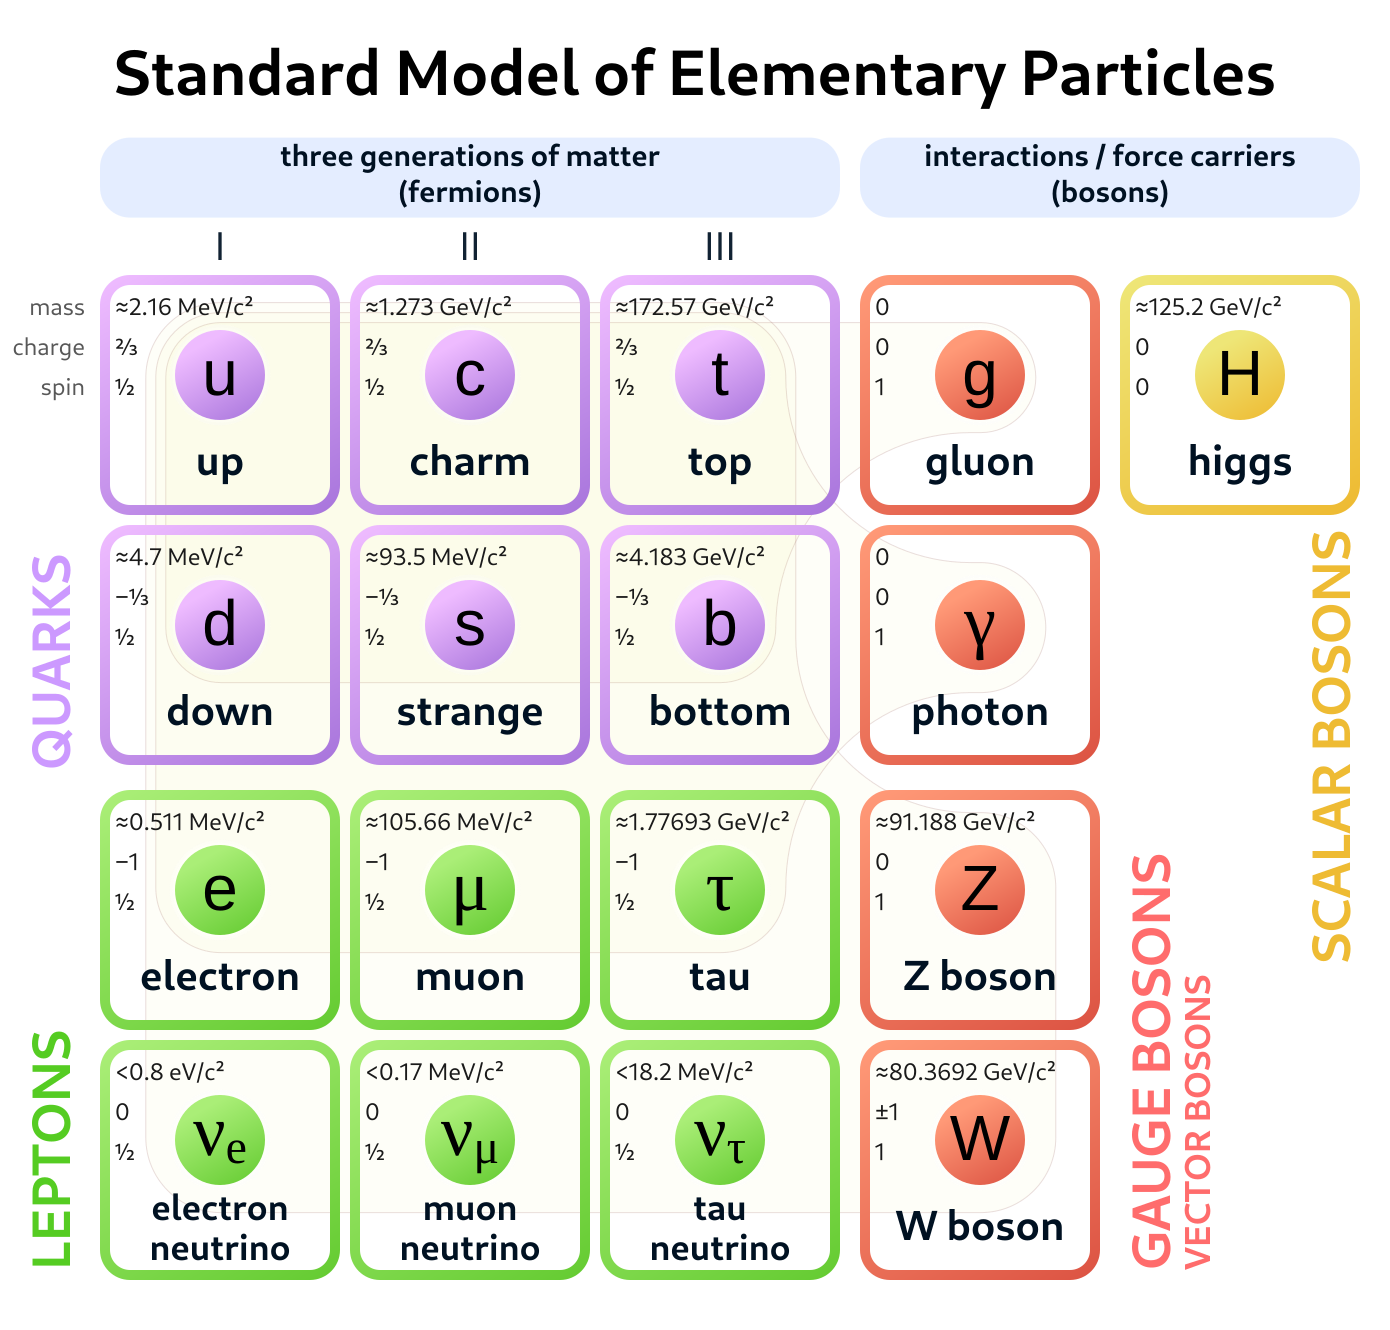
\includegraphics[width=0.8\textwidth]{figures/standard_model.png}\caption{Elementary particles of the Standard Model: 12 fundamental fermions and 5 fundamental bosons. Brown loops indicate which bosons (red) couple to which fermions (purple and green).}
\label{fig:smcontent}
\end{center}
\end{figure}

A compact and efficient mathematical formulation of the SM is achieved through the Lagrandian formalism. The dynamics and kinematics of the underlying fields are encoded in a Lagrangian density constructed to be invariant under both the global symmetries of special relativity (embodied in the Poincaré group) and local gauge transformations. The requirement for local gauge invariance leads to the symmetry group
\begin{equation}
\mathrm{SU}_C(3) \times \mathrm{SU}_L(2) \times \mathrm{U}_Y(1):
\label{SM_symmetry_group}
\end{equation}
$\mathrm{SU}_C(3)$ governs quantum chromodynamics (QCD), the theory of the strong interaction, acting on the gluon fields and all the particles that carry color charge; $\mathrm{SU}_L(2)$ is associated with the weak isospin and acts on the left-handed fermions as well as on the Higgs field; $\mathrm{U}_Y(1)$ corresponds to the weak hypercharge, and together with $\mathrm{SU}_L(2)$ forms the electroweak sector, giving rise to the electric charge after the electroweak symmetry breaking.

The SM provides a precise description of the particle content and their interactions, and has provided an extraordinary predictive power across a wide range of energies. Besides, despite its success, the SM is generally thought to be an effective theory as it leaves unanswered several fundamental questions, such as the incorporation of a quantum theory of gravity, the hierachy of mass scales, the origin of neutrino masses and the nature of dark matter, suggesting that the SM is not the ultimate theory of fundamental interactions. These limitations have motivated the search for extensions beyond the SM. Among these, supersymmetry (SUSY) has attracted significant attention. By postulating a symmetry between bosons and fermions, SUSY offers potential solutions to most of the SM's shortcomings, although experimental confirmation of supersymmetric partners have yet been observed.

This chapter provides an overview of the SM's main features, including its particle content and the construction of the Lagrangian, and discusses the shortcomings that motivate the exploration of extensions such as SUSY. Natural units, with $c=\hbar=1$, will be adopted throughout.
 
\section{Gauge Invariance in QFT}
\label{gauge_inv}

The principle of gauge invariance is cleanly illustrated by quantum electrodynamics (QED), the quantum field theory based on the $\mathrm{U}(1)$ symmetry group that describes electromagnetic interactions. Consider the Dirac fermionic field $\psi(x)$ with its adjoint defined as $\bar{\psi}(x)=\psi^\dagger(x)\gamma^0$. Under a local $\mathrm{U}(1)$ phase transformation, the field transforms as
\begin{equation}
\psi(x) \to \psi^\prime(x)=\mathrm{e}^{iq\chi(x)}\psi(x),
\end{equation}
where the phase $q\chi(x)$ may vary from point to point in space-time. If one applies this transformation to the free Dirac Lagrangian density
\begin{equation}
\mathcal{L}=\bar{\psi}(x)(i\gamma^\mu\partial_\mu-m)\psi(x),
\end{equation}
the Lagrangian transforms into
\begin{equation}
\mathcal{L}^\prime=\bar{\psi}^\prime(x)(i\gamma^\mu\partial_\mu-m)\psi^\prime(x).
\end{equation}
A straightforward calculation shows that
\begin{equation}
\mathcal{L}^\prime=\mathcal{L}-q\bar{\psi}(x)\gamma^\mu
(\partial_\mu\chi(x))\psi(x),
\end{equation}
revealing an extra term proportional to $\partial_\mu\chi(x)$, indicating that the free Dirac Lagrangian is not ivariant under local $\mathrm{U}(1)$ transformations. In order to restore local gauge invariance, the derivative $\partial_\mu$ must be replaced by the covariant derivative $D_\mu$, defined as
\begin{equation}
D_\mu=\partial_\mu+iqA_\mu(x),
\end{equation}
where $A_\mu(x)$ is a new gauge field. To have consistency under the local phase transformation, it is required that $A_\mu(x)$ transforms according to
\begin{equation}
A_\mu(x) \to A_\mu^\prime(x)=A_\mu - \partial_\mu\chi(x).
\end{equation}
The Dirac Lagrangian then beomes
\begin{equation}
\mathcal{L}=\bar{\psi}(x)(i\gamma^\mu D_\mu -m)\psi(x)=\bar{\psi}(x)(i\gamma^\mu -q\gamma^\mu A_\mu(x)-m)\psi(x).
\end{equation}
The new term $q\bar{\psi}(x)\gamma^\mu A_\mu(x)\psi(x)$ describes the interaction between the charged Dirac field and the electromagnetif field, i.e. identifying $A_\mu$ as the mediator of the electromagnetic interaction (the photon) and $q$ as the electric charge.

The full QED Lagrangian is obtained by adding the gauge-invariant kinetic term for the electromagnetic field:
\begin{equation}
\mathcal{L}=\bar{\psi}(x)(i\gamma^\mu D_\mu -m)\psi(x)-\frac{1}{4}F_{\mu\nu}(x)F^{\mu\nu}(x),
\end{equation}
where the field strenght tensor is defined as
\begin{equation}
F_{\mu\nu}(x)=\partial_\mu A_\nu(x)-\partial_\nu A_\mu(x).
\end{equation}
Thus, the requirement of local $\mathrm{U}(1)$ invariance implies the existence of a spin-1 gauge field $A_\mu(x)$, whose coupuling with the Dirac field not only ensures gauge invariance but also naturally represents the mediator of the electromagnetic interaction, the photon.

\section{Quantum Chromo Dynamics}
\label{sec:qcd}

Quantum chromodynamics (QCD) is the gauge theory of the color symmetry group $\mathrm{SU}_C(3)$ and describes the strong interaction between quarks and gluons. Quarks and gluons are the fundamental constituents of hadrons -composit particles (such as baryons and mesons) bound together by the strong force. Only particles carrying non-zero color charge interact strongly; therefore, colorless leptons do not feel the strong interaction.

There are three color charges, conventionally labeled $r$, $g$, and $b$, corresponding to three orthogonal states in the $\mathrm{SU}(3)$ color space. Each quark flavor forms a triplet in the fundamental representation of $\mathrm{SU}(3)$, while antiquarks belong to the conjugate representation, carrying the anticolors $\bar{r}$, $\bar{g}$, and $\bar{b}$. The strong interaction is mediated by eight massless gluons associated with the eight generators of $\mathrm{SU}(3)$, an exact symmetry that ensures invariance under unitary transformations in color space.

The QCD Lagrangian density is given by:
\begin{equation}
\mathcal{L}_{QCD}=\sum_q \bar{\psi}_{q,a} (i\gamma_\mu D^\mu_{ab} -m_q \delta_{ab})\psi_{q,b}-\frac{1}{4}F_{\mu\nu}^A F^{\mu\nu}_A,
\end{equation}
where the sum runs over quark flavors $q$. Here, $\gamma^\mu$ are the Dirac matrices, $\psi_{q,a}$ is the quark field of flavor $q$ and mass $m_q$, with the color index $a=1,2,3$, and $\bar{\psi_{q,a}}$ its Dirac adjoint.

The gauge covariant derivative $D^\mu_{ab}$ is defined as:
\begin{equation}
D^\mu_{ab}=\delta_{ab}\partial^\mu + ig_S (t^A)_{ab}G^\mu_A,
\end{equation}
where $g_S$ is the strong coupling constant, $G^\mu_A$ (with $A=1,...,8$) are the gluon fields, and the matrices $t^A_{ab}=\lambda^A_{ab}/2$ are the generators of $\mathrm{SU}(3)$, with $\lambda^A$ the Gell-Mann matrices. These generators satisfy the commutation relation:
\begin{equation}
[t_A,t_B]=if_{ABC}t_C,
\end{equation}
with $f_{ABC}$ being the totally anstisymmetric structure constants of $\mathrm{SU}(3)$.

The gluon field strength tensor is given by:
\begin{equation}
F_{\mu\nu}^A=\partial_\mu G_\nu^A - \partial_\nu G_\mu^A - g_S f_{ABC} G_\mu^B G_\nu^C.
\end{equation}

Color charge conservation requires that gluons themselves carry color. Since quarks carry one of the three colors and antiquarks one of the three anticolors, each gluon must carry both a color and an anticolor. Although there are nine possible color-anticolor independend combinations, only eight correspond to the independent physical gluon states, forming an octet. One way these states can be represented is the following:
\begin{equation}
r\bar{g}, \quad g\bar{r}, \quad r\bar{b}, \quad b\bar{r}, \quad g\bar{b}, \quad b\bar{g}, \quad \frac{1}{\sqrt{2}}(r\bar{r}-g\bar{g}), \quad \frac{1}{\sqrt{6}}(r\bar{r}+g\bar{g}-2b\bar{b}).
\end{equation}
In addition, there exist another independent combination,
\begin{equation}
\frac{1}{\sqrt{3}}(r\bar{r}+b\bar{b}+g\bar{g}),
\end{equation}
which is inveriant under $\mathrm{SU}(3)$ rotations. However, $\mathrm{SU}(3)$ is defined as the group of $3\times 3$ unitary matrices with determinant one, which restricts its generators to be traceless -yielding only eight independent generators (the Gell-Mann matrices). Including a ninth generator would extend the symmetry to $\mathrm{U}(3)$, and the additional generator would correspond to a color singlet state. Since QCD is based on $\mathrm{SU}(3)$, only the eight color-octet gluons are physical. Moreover, the absence of a physical color-neutral gluon is constistent with the observation that hadrons, which are color singlets, do not experience long-range interactions.

Ultimately, QCD not only provides a detailed description of quark and gluon dynamics but also explains why only color-neutral states are observed in nature. 


\subsection{Color Confinment, Asymptotic freedom, Hadronization and Jets}
\label{subsec:confinment}


Quarks and gluons are the fundamental fields of QCD, yet free quarks and gluons have never been observed. This is due to color confinment, which requires that only color-neutral (singlet) states can exist as free particles. In practice, quarks are always bound into hadrons, composite particles such as baryons (typically three-quark states like proton and neutrons) and mesons (quark-antiquark pairs). Color singlet states made up of gluons only (``glueballs'') are also consistent with color confinment, but have so far not been experimentally observed.

There is currently no analytical proof of color confinement, though a qualitative picture can be obtained by considering two quarks being pulled apart. As they separate, the quarks interact by exchanging virtual gluons, which themselves carry color. This leads to gluon self-interactions and the formation of a narrow flux tube with constant energy density between the quarks. Consequently, the energy stored in the gluon field increases linearly with distance, making it energetically impossible to isolate individual quarks. Instead, when the energy in the flux tube becomes sufficiently high, it is more favorable to create a new quark-antiquark pair, a process knows as hadronization. In high-energy experiments, this mechanism results in the formation of narrow hadronic jets that reflect the original quark directions.

In contrast to the strong coupling at low energies responsible for confinement, QCD exhibits asymptotic freedom: the strong interaction becomes weaker at higher energy scales, allowing perturbative calculations. This behavior originates from vacuum polarization effects in QCD. Virtual quark-antiquark pairs tend to screen a physical color charge, while virtual gluon pairs, carrying both color and anticolor, produce an anti-screening effect. For QCD, with three colors ($N_C=3$) and six quark flavors ($N_f=6$), anti-screening dominates, so that the effective coupling $\alpha_S$ decreases with increasing momentum transfer $Q^2$. In perturbative QCD the running coupliong is expressed as
\begin{equation}
\alpha_S(Q^2)=\frac{\alpha_S(Q^2)}{1+\beta_0\alpha_S(\mu^2)\mathrm{ln}\left( \frac{Q^2}{\mu^2}\right)},
\end{equation}
with
\begin{equation}
\beta_0=\frac{11N_C -2N_f}{12\pi}.
\end{equation}
At high energies, quarks behave as quasi-free particles, while at low energies $\alpha_S$ grows until it diverges at the scale $\Lambda_{QCD} \sim 332 \pm 17$ MeV, marking the onset of confinement.

Thus, QCD displayis a dual nature: asymptotic freedom at high energy permits a perturbative treatment of quark gluon interactions, whereas at low energies, color confinement ensures that only color-neutral hadrons are observed.

\section{Electroweak Theory}
\label{ew_theory}

The electroweak theory unifies the electromagnetic and weak interactions under the gauge group
\begin{equation}
\mathrm{SU}_L(2) \times \mathrm{U}_Y(1)
\end{equation}
with the gauge fields $W_\mu^1$, $W_\mu^2$, and $W_\mu^3$ associated with $\mathrm{SU}(2)$ (carrying weak isospin) and $B_\mu$ associated with $\mathrm{U}(1)$ (carrying hypercharge). Its Lagrandian density is given by:
\begin{equation}
\mathcal{L}_{EW}=-\frac{1}{4}\sum_{A=1}^3 F_{\mu\nu}^A F_A^{\mu\nu}-\frac{1}{4}B_{\mu\nu}B^{\mu\nu}+\sum_j \left[ \bar{\psi}_L^j i \gamma^\mu D_\mu \psi_L^j + \bar{\psi}_R^j i \gamma^\mu D_\mu \psi_R^j \right],
\end{equation}
where the index $j$ runs over the three fermion generations. The $\mathrm{SU}(2)$ field strength tensor is
\begin{equation}
F_{\mu\nu}^A=\partial_\mu W^A_\nu-\partial_\nu W_\mu^A-g_W \epsilon_{ABC} W_\mu^B W_\nu^C,
\end{equation}
and the $\mathrm{U}(1)$ tensor is
\begin{equation}
B_{\mu\nu}=\partial_\mu B_\nu - \partial_\nu B_\mu.
\end{equation}
Here, $g_W$ is the $\mathrm{SU}(2)$ coupling constant and $\epsilon_{ABC}$ is the totally antisymmetric Levi-Civita symbol.

The fermion fields are split into left- and right-handed components. For a Dirac field $\psi$, chirality is defined by
\begin{equation}
\gamma_5= i \gamma^0\gamma^1\gamma^2\gamma^3,
\end{equation}
with eigenvalues $-1$ for left-handed (LH) and $+1$ for right-handed (RH) states. The projections are given by
\begin{equation}
\psi_L=\frac{1-\gamma_5}{2}\psi, \quad \psi_R=\frac{1+\gamma_5}{2}\psi,
\end{equation}
and similarly for the adjoints. Since only the LH particles (and RH antiparticles) participate in charged weak interactions, LH fields are arranged in $\mathrm{SU}(2)$ doublets, while RH fields are $\mathrm{SU}(2)$ singlets.

The covariant derivative is defined as
\begin{equation}
D_\mu = \partial_\mu + ig_W \sum_{A=1}^3 T^A W_\mu^A+ ig^\prime \frac{Y}{2}B_\mu,
\end{equation}
where $T^A$ are the $\mathrm{SU}(2)$ generators satisfying
\begin{equation}
[T^A,T^B]=i\epsilon_{ABC}T^C,
\end{equation}
and $Y$ is the weak hypercharge. The electric charge $Q$ is given by the Gell-Mann-Nishijima relation,
\begin{equation}
Q=T^3+\frac{1}{2}Y.
\end{equation}
For the three fermion families, the LH weak isospin doublets are
\begin{equation}
\binom{\nu_\ell}{\ell^-}_L \quad \mathrm{and} \quad \binom{q_u}{q_d^\prime}_L,
\end{equation}
while the RH singlets are $l_R^-$, $q_{uR}$, and $q_{dR}^\prime$. Here, $q_d^\prime$ denotes the weak eigenstates, which are mixtures of the mass eigenstates $q_d$ via the Cabibbo-Kobayashi-Maskawa matrix.

Charged current (CC) interactions arise from the fields $W_\mu^1$ and $W_\mu^2$, which combine to form the charged bosons:
\begin{equation}
W_\mu^\pm = \frac{1}{\sqrt{2}}(W_\mu^1 \mp i W_\mu^2),
\end{equation}
with the corresponding ladder operators $T^\pm = T^1 \mp iT^2$. The CC Lagrangian is
\begin{equation}
\mathcal{L}_{CC}= \frac{g_W}{2\sqrt{2}} \sum_j \left[ \bar{\psi}_L^j \gamma^\mu (1-\gamma_5)(T^+W_\mu^+ + T^- W_\mu^-)\psi_L^j\right],
\end{equation}
which exhibits a pure V-A structure (i.e. ``pure vector minus axial-vector''), coupling only to LH fermions and RH antifermions.

Neutral currents (NC) involve the neutral bosons, which arise as orthogonal combinations of $W_\mu^3$ and $B_\mu$:
\begin{equation}
\begin{cases}
      A_\mu = \cos \theta_W B_\mu + \sin \theta_W W_\mu^3 \\
      Z_\mu = -\sin \theta_W B_\mu + \cos \theta_W W_\mu^3
    \end{cases},
\end{equation}
with the weak mixing angle $\theta_W$. $Z_\mu$ is identified with the mediator of the weak NC and $A_\mu$ with the photon. The photon couples universally with strength $e$, where
\begin{equation}
e=g_W\sin \theta_W=g^\prime \cos \theta_W \implies \frac{g^\prime}{g_W}= \tan \theta_W.
\end{equation}
The NC Lagrangian is given by
\begin{equation}
\mathcal{L}_{NC}= \frac{g_W}{2 \cos \theta_W} \sum_j \bar{\psi}^j \gamma^\mu \left( g_V^j - g_A^j \gamma_5\right) \psi^j Z_\mu,
\end{equation}
with vector and axial couplings defined as
\begin{equation}
g_V^j = T^{3j}-2Q^j \sin^2\theta_W, \quad g_A^j = T^{3j}.
\end{equation}
Alternatively, defining
\begin{equation}
g_L^j = \frac{1}{2}(g_V^j+g_A^j) \quad \mathrm{and} \quad g_R^j=\frac{1}{2}(g_V^j-g_A^j),
\end{equation}
the NC interaction can be written as
\begin{equation}
\mathcal{L}_{NC}=\frac{g_W}{2 \cos \theta_W} \sum_j \bar{\psi}^j \gamma^\mu \left[ g_L^j (1-\gamma_5) + g_R^j(1+\gamma_5)\right] \psi^j Z_\mu,
\end{equation}
demonstrating that, unlike the charged currents, both LH and RH components participate in neutral interactions.

In summary, the electroweak theory, with its chiral structure and well-defined gauge interactions, successfully unifies electromagnetic and weak forces while predicting the observed phenomena of charged and neutral current interactions.


\section{Higgs Sector}


The electroweak model described in Section \ref{ew_theory} unifies electromagnetic and weak interactions by introducing gauge bosons as force mediators through the requirement of gauge invariance. This invariance ins mantained by replacing the partial derivative $\partial_\mu$ with the covariant derivative $D_\mu$, which introduces new vector fields. However, in gauge theories it is not permissible to include explicit mass terms for these gauge bosons, as such terms would break local gauge invariance. For example, in QED (discussed in Section \ref{gauge_inv}), a poton mass term
\begin{equation}
\frac{1}{2}m_\gamma^2 A_\mu A^\mu
\end{equation}
would transform under
\begin{equation}
A_\mu \to A_\mu^\prime = A_\mu - \partial_\mu \chi
\end{equation}
to
\begin{equation}
\frac{1}{2} m_\gamma^2 (A_\mu - \partial_\mu \chi)(A^\mu - \partial^\mu \chi),
\end{equation}
which clearly does not equal the original mass term. Thus, the $\mathrm{U}(1)$ gauge symmetry of QED, as well as the $\mathrm{SU}(3)$ of QCD and the $\mathrm{SU}(2)$ of weak isospin, requires massless gauge bosons. This is acceptable for photons and gluons, but poses a problem for the electroweak theory where the $W^\pm$ and $Z$ bosons are experimentally known to be massive.

Similarly, explicit fermion mass terms of the form
\begin{equation}
-m_f (\bar{\psi}_R\psi_L + \bar{\psi}_L \psi_R)
\end{equation}
are not allowed, because the left-handed fermions transform as $\mathrm{SU}(2)$ doublets while the right-handed ones are singlets, making such mass terms non-invariant under $\mathrm{SU}(2)\times \mathrm{U}(1)$.

The solution to this problem is provided by spontaneous symmetry breaking via the Higgs mechanism. In this framework, the $\mathrm{SU}(2)\times \mathrm{U}(1)$ symmetry remains intact in the Lagrangian, but the vacuum state does not respect the symmetry. Interactions with the scalar Higgs field then generate masses for the $W^\pm$ and $Z$ bosons, as well as for the fermions, without explicitly breaking the gauge invariance of the theory. This mechanism, introduced by Higgs, Brout, Englert and others in the 1960s, is the cornerstone of the SM.


\subsection{Spontaneous Symmetry Breaking}

Consider a complex scalar field
\begin{equation}
\phi = \frac{1}{\sqrt{2}}(\phi_1+i\phi_2)
\end{equation}
with potential
\begin{equation}
V(\phi) = \mu^2 \phi^* \phi + \lambda (\phi^*\phi)^2.
\end{equation}
Its Lagrangian density is
\begin{equation}
\mathcal{L}=(\partial_\mu \phi)^*(\partial^\mu \phi) - V(\phi).
\end{equation}
Expressed in terms of the real fields $\phi_1$ and $\phi_2$, it becomes
\begin{equation}
\mathcal{L}=\frac{1}{2}(\partial_\mu\phi_1)^2 + \frac{1}{2}(\partial_\mu \phi_2)^2 - \frac{1}{2}\mu^2 (\phi_1^2+\phi^2_2) - \frac{1}{4}\lambda (\phi_1^2+\phi_2^2)^2.
\end{equation}
This Lagrangian is invariant under global $\mathrm{U}(1)$ transformations, $\phi\to\mathrm{e}^{i\alpha}\phi$, since $\phi^*\phi$ is unchanged.

For $\lambda>0$ the potential is bounded from below, and its minimum depends on the sign of $\mu^2$:
\begin{itemize}
\item[-] if $\mu^2>0$, the minimum is at $\phi_1=\phi_2=0$,
\item[-] if $\mu^2<0$, the minimum is not unique but lies on a circle defined by
\begin{equation}
\phi_1^2+\phi_2^2=\frac{-\mu^2}{\lambda} = v^2,
\end{equation}
\end{itemize}
with $v$ the vacuum expectation value (VEV). Choosing a specific vacuum state (say, $\phi_1=v$ and $\phi_2=0$) spontaneously breaks the global $U(1)$ symmetry.

Expanding around the chosen vacuum,
\begin{equation}
\phi_1(x)=v+\eta(x), \quad \phi_2(x)=\xi(x),
\end{equation}
so that
\begin{equation}
\phi(x)=\frac{1}{\sqrt{2}} \left( v + \eta(x) + i \xi(x)\right),
\end{equation}
the Lagrangian becomes
\begin{equation}
\mathcal{L}=\frac{1}{2}(\partial_\mu\eta)^2 + \frac{1}{2}(\partial_\mu\xi)^2 - \frac{1}{2}(2\lambda v^2)\eta^2 -V_{int}(\eta,\xi),
\end{equation}
where the quadratic term in $\eta$ gives it a mass $m_\eta=\sqrt{2\lambda v^2}$ while $\xi$ remains massless. The massless scalar $\xi$ is the Goldstone boson, arising from the broken continuous symmetry.

This spontaneous symmetry breaking mechanism can be embedded in a local $\mathrm{U}(1)$ gauge theory. In that case, one replaces the ordinary derivative with the covariant derivative
\begin{equation}
D_\mu = \partial_\mu + igB_\mu,
\end{equation}
where $B_\mu$ is a massless gauge field that transforms as
\begin{equation}
B_\mu \to B_\mu^\prime= B_\mu - \partial_\mu \alpha(x),
\end{equation}
and the Lagrangian becomes
\begin{equation}
\mathcal{L}=-\frac{1}{4}F_{\mu\nu}F^{\mu\nu}+(D_\mu\phi)^*(D^\mu\phi) - \mu^2\phi^*\phi - \lambda(\phi^*\phi)^2,
\end{equation}
with $F_{\mu\nu}=\partial_\mu B_\nu - \partial_\nu B_\mu$.

For $\mu^2<0$ the field acquires a VEV, and writing
\begin{equation}
\phi(x) = \frac{1}{\sqrt{2}} \left( v + \eta(x9 +i\xi(x)\right),
\end{equation}
one finds, besides the kinetic and potential terms for $\eta$ and $\xi$, a gauge-dependent mixing term $gvB_\mu\partial^\mu\xi$ and a mass term for the gauge field, $\frac{1}{2}g^2v^2B_\mu B^\mu$. By choosing the unitary gauge, where one performs a gauge transformation to set $\xi(x)=0$, the Lagrangian simplifies to
\begin{equation}
\mathcal{L}=\frac{1}{2}(\partial_\mu\eta)^2 - \lambda v^2\mu^2 - \frac{1}{4}F_{\mu\nu}F^{\mu\nu}+\frac{1}{2}g^2v^2B_\mu B^\mu + \mathrm{interaction terms}.
\end{equation}
Thus, the spetrum consists of a massive scalar field $\eta$ with $m_\eta=\sqrt{2\lambda v^2}$ (the Higgs boson) and a massive gauge boson $B_\mu$ with mass $m_B=gv$. The original Goldstone boson $\eta$ has been ``eaten'' by the gauge field, becoming its longitudilal polarization. This is the essence of the Higgs mechanism.


\subsection{The Higgs Mechanism in the Standard Model}

The Higgs mechanism is incorporated into the SM to spontaneously break the $SU_L(2) \times U_Y(1)$ electroweak symmetry down to the electromagnetic $U_\mathrm{em}(1)$ symmetry, generating masses for the $W^\pm$ and $Z$ bosons while keeping the photon massless.

To preserve the fundamental $SU_L(2) \times U_Y(1)$ gauge symmetry, the simplest approach introduces a complex scalar $SU_L(2)$ doublet with hypercharge $Y = +1$:
\begin{equation}
\phi = \begin{pmatrix} \phi^+ \\ \phi^0 \end{pmatrix} = \frac{1}{\sqrt{2}} \begin{pmatrix} \phi_1 + i\phi_2 \\ \phi_3 + i\phi_4 \end{pmatrix},
\end{equation}
where $\phi^+$ carries electric charge $+1$ and $\phi^0$ is neutral.

The Higgs potential is given by
\begin{equation}
V(\phi) = \mu^2 \phi^\dagger \phi + \lambda(\phi^\dagger \phi)^2,
\end{equation}
which for $\lambda > 0$ and $\mu^2 < 0$ has degenerate minima satisfying
\begin{equation}
\phi^\dagger \phi = -\frac{\mu^2}{2\lambda} = \frac{v^2}{2},
\end{equation}
where $v$ is the vacuum expectation value (VEV).

To break $SU_L(2) \times U_Y(1)$ while preserving $U_{em}(1)$, only the neutral component can acquire a non-zero VEV. Choosing the vacuum state and expanding in the unitary gauge:
\begin{equation}
\phi(x) = \frac{1}{\sqrt{2}} \begin{pmatrix} 0 \\ v + h(x) \end{pmatrix},
\end{equation}
where $h(x)$ is the physical Higgs field. In this way, the symmetry is broken such that the electromagnetic generator $Q = T^3+\frac{Y}{2}$ remains unbroken.

The gauge boson masses are generated by the kinetic term $(D_\mu\phi)^\dagger(D^\mu\phi)$ in the Lagrangian, where the covariant derivative is given by
\begin{equation}
D_\mu = \partial_\mu + ig_W \sum_{A=1}^3 T^A W_\mu^A + ig^\prime \frac{Y}{2}B_\mu.
\end{equation}
Expanding this term yields mass terms for the gauge bosons:
\begin{equation}
\mathcal{L}_{\text{mass}} = \frac{1}{8}v^2 \left[ 2g_W^2(W^{+\mu}W^-_\mu) + (W^{3\mu}, B^\mu) \begin{pmatrix} g_W^2 & -g_Wg' \\ -g_Wg' & g'^2 \end{pmatrix} \begin{pmatrix} W^3_\mu \\ B_\mu \end{pmatrix} \right].
\end{equation}

In particular, the charged $W^\pm$ fields, defined as
\begin{equation}
W^\pm_\mu = \frac{1}{\sqrt{2}}(W_\mu^1 \mp iW_\mu^2),
\end{equation}
acquire masses $m_W=\frac{1}{2}vg_W$.
The neutral fields $W_\mu^3$ and $B_\mu$ mix; diagonalization yields the massless photon
\begin{equation}
A_\mu = \frac{g^\prime W_\mu^3 + g_W B_\mu}{\sqrt{g_W^2+g^{\prime 2}}},
\end{equation}
and the $Z$ boson
\begin{equation}
Z_\mu = \frac{g_W W_\mu^3 - g^\prime B_\mu}{\sqrt{g_W^2+g^{\prime 2}}},
\end{equation}
with mass $m_Z = \frac{1}{2}v\sqrt{g_W^2+g^{\prime 2}}$.

The Higgs boson mass, $m_h = \sqrt{2\lambda}v$, is determined by the quadratic term in the scalar potential.

Fermion masses arise through Yukawa interactions with the Higgs doublet. Since only $\phi^0$ acquires a VEV, generating masses for up-type quarks requires the charge-conjugate doublet:
\begin{equation}
\tilde{\phi} = i\sigma_2 \phi^* = \begin{pmatrix} \phi^{0*} \\ -\phi^- \end{pmatrix}.
\end{equation}

The Yukawa Lagrangian is
\begin{equation}
\mathcal{L}_{\text{Yukawa}} = -\sum_{i,j} \left[ Y^e_{ij} \bar{L}_i \phi e_{R,j} + Y^d_{ij} \bar{Q}_i \phi d_{R,j} + Y^u_{ij} \bar{Q}_i \tilde{\phi} u_{R,j} \right] + \text{h.c.},
\end{equation}
where $L_i$ and $Q_i$ denote the lepton and quark $SU_L(2)$ doublets of generation $i$, and $Y^{e,d,u}$ are the Yukawa coupling matrices. After symmetry breaking, fermion masses are
\begin{equation}
m_f = \frac{Y_f v}{\sqrt{2}}.
\end{equation}

Therefore, the Higgs mechanism provides a unified framework for mass generation in the SM: the $W^\pm$ and $Z$ bosons acquire mass through their coupling to the Higgs VEV, fermions obtain mass via Yukawa couplings, and the photon remains massless as required by the unbroken $U_\mathrm{em}(1)$ symmetry.


\section{Shortcomings of the Standard Model}

The SM, while being the most successful theory to date for describing fundamental particles and their interactions up to the TeV scale, is nonetheless believed to be an effective field theory that must be embedded in a more fundamental framework. Several theoretical and experimental observations point to physics beyond the Standard Model (BSM).

\textbf{Gravity.} The SM does not incorporate general relativity. At the Planck scale ($M_P \sim 10^{19}$ GeV), quantum gravitational effects become important, yet no consistent quantum theory of gravity exists within the SM. The gravitational interaction is fundamentally different from the gauge interactions, and attempts to quantize gravity using standard QFT methods lead to a non-renormalizable theory.


\textbf{Hierarchy problem.} The Higgs mass receives quadratic corrections from quantum loops:
\begin{equation}
\delta m_h^2 \sim \frac{\Lambda^2}{16\pi^2} \left( 6\lambda + \frac{3}{2}(g^2 + g'^2) - 12y_t^2 \right),
\end{equation}
where $\Lambda$ is the cutoff scale and $y_t$ is the top Yukawa coupling. If there is no new physics before the Planck scale, i.e. $\Lambda \sim M_P$, these corrections are $\mathcal{O}(10^{30})$ times larger than the physical Higgs mass, requiring extreme fine-tuning to maintain $m_h \sim 125$ GeV.

\textbf{Dark matter.} Cosmological observations from galaxy rotation curves, gravitational lensing, and the cosmic microwave background indicate that approximately 27\% of the universe's energy density consists of dark matter. This matter interacts gravitationally but not electromagnetically, and the SM contains no viable dark matter candidate.

\textbf{Neutrino masses.} Neutrino oscillation experiments demonstrate that neutrinos have non-zero masses and mix between flavors, contradicting the SM prediction of massless neutrinos. The observed mass scale $m_\nu \lesssim 0.1$ eV is orders of magnitude smaller than other fermion masses, suggesting a different mass generation mechanism such as the seesaw mechanism.

\textbf{Matter-antimatter asymmetry.} The observed baryon asymmetry of the universe, quantified as $n_B/n_\gamma \sim 6 \times 10^{-10}$, requires CP violation beyond that present in the CKM matrix. The three Sakharov conditions for baryogenesis (baryon number violation, C and CP violation, and departure from thermal equilibrium) cannot be simultaneously satisfied within the SM.

\textbf{Strong CP problem.} The QCD Lagrangian allows for a CP-violating term
\begin{equation}
\mathcal{L}_{\theta} = \frac{\theta g_s^2}{32\pi^2} G^A_{\mu\nu} \tilde{G}^{A\mu\nu},
\end{equation}
where $\tilde{G}^{A\mu\nu} = \frac{1}{2}\epsilon^{\mu\nu\rho\sigma}G^A_{\rho\sigma}$ is the dual field strength tensor. Experimental bounds on the neutron electric dipole moment constrain $|\theta| < 10^{-10}$, requiring unexplained fine-tuning of this dimensionless parameter.

\textbf{Gauge coupling unification.} The three SM gauge couplings evolve differently with energy scale according to their renormalization group equations. When extrapolated to high energies, they do not unify at a single scale, theoretically suggesting the SM gauge group may be embedded in a larger unified structure.

\subsection{Supersymmetry}

Among the many proposed BSM theories, supersymmetry (SUSY) has been one of the most popular and widely studied. SUSY postulates a fundamental symmetry between bosons and fermions, predicting that each SM particle has a superpartner differing by spin-1/2, where bosonic superpartners are named with a prefix ``s-'' (e.g. squarks) and fermionic ones with a suffix ``-ino'' (e.g. gluinos). This symmetry, if realized in nature, would represent the first extension of spacetime symmetries beyond the Poincaré group. This is a unique feature of SUSY, as it is the only known theoretical framework that predicts the Poincaré symmetries as part of a larger, unified mathematical structure.

The supersymmetry algebra extends the Poincaré algebra by introducing anticommuting spinorial generators $Q_\alpha$ and their conjugates $\bar{Q}_{\dot{\alpha}}$. These generators satisfy the fundamental anticommutation relation:
\begin{equation}
\{Q_\alpha, \bar{Q}_{\dot{\beta}}\} = 2\sigma^\mu_{\alpha\dot{\beta}} P_\mu,
\end{equation}
where $P_\mu$ is the four-momentum operator, $\sigma^\mu = (1, \vec{\sigma})$ with $\vec{\sigma}$ being the Pauli matrices, and $\alpha, \dot{\beta}$ are two-component spinor indices. All other anticommutators vanish: $\{Q_\alpha, Q_\beta\} = \{\bar{Q}_{\dot{\alpha}}, \bar{Q}_{\dot{\beta}}\} = 0$.


Under a SUSY transformation, fields transform into their superpartners. The transformation is parameterized by an infinitesimal anticommuting spinor $\epsilon$. As a basic example, consider a supermultiplet containing a complex scalar field $\phi$ and its fermionic superpartner $\psi$ (a two-component Weyl spinor). The SUSY transformation acts on these fields as:
\begin{align}
\phi &\to \phi + \epsilon \psi, \\
\psi &\to \psi + i\sigma^\mu \bar{\epsilon} \partial_\mu \phi + F\epsilon,
\end{align}
where $F$ is an auxiliary field (a non-propagating field with no kinetic term) that ensures the closure of the SUSY algebra. This means that the transformation turns bosons into fermions and vice versa, relating particles of different spin within the same supermultiplet.


In the Minimal Supersymmetric Standard Model (MSSM), each SM particle is part of a supermultiplet. The particle content doubles:

\begin{itemize}
\item Quarks $q$ $\to$ squarks $\tilde{q}$ (spin-0)
\item Leptons $\ell$ $\to$ sleptons $\tilde{\ell}$ (spin-0)
\item Gauge bosons $\to$ gauginos: photino $\tilde{\gamma}$, winos $\tilde{W}^\pm$, zino $\tilde{Z}$, gluinos $\tilde{g}$ (spin-1/2)
\item Higgs bosons $\to$ higgsinos $\tilde{H}$ (spin-1/2)
\end{itemize}

The MSSM requires two Higgs doublets, $H_u$ and $H_d$, unlike the single doublet in the SM. This is necessary because: the superpotential must be holomorphic (containing only fields, not their conjugates), preventing a single Higgs from giving mass to both up-type and down-type fermions; anomaly cancellation requires the fermionic higgsinos to come in vector-like pairs.

If SUSY were exact, superpartners would have identical masses to their SM counterparts. Since no superpartners have been observed so far, SUSY must be broken. The breaking mechanism introduces soft SUSY-breaking terms that preserve the cancellation of quadratic divergences:
\begin{equation}
\mathcal{L}_{\text{soft}} = -\frac{1}{2} \sum_a M_a \lambda^a \lambda^a - \sum_{i,j} m^2_{ij} \tilde{\phi}_i^* \tilde{\phi}_j - \left( \sum_{i,j,k} A_{ijk} y_{ijk} \tilde{\phi}_i \tilde{\phi}_j \tilde{\phi}_k + \text{h.c.} \right),
\end{equation}
where $M_a$ are gaugino masses, $m^2_{ij}$ are scalar mass matrices, and $A_{ijk}$ are trilinear couplings.

SUSY addresses several SM shortcomings:

\textbf{Hierarchy problem.} Quadratic divergences from fermion loops are exactly canceled by their scalar superpartners. For instance, the top quark contribution to the Higgs mass is canceled by stop (top squark) loops:
\begin{equation}
\delta m_h^2|_{\text{top}} + \delta m_h^2|_{\text{stop}} = \frac{3y_t^2}{8\pi^2} \left( m_{\tilde{t}}^2 - m_t^2 \right) \ln\left(\frac{\Lambda^2}{m_{\tilde{t}}^2}\right),
\end{equation}
which is only logarithmically divergent rather than quadratically divergent. Even with $m_{\tilde{t}} \sim$ TeV (as required by current experimental bounds), this represents a significant improvement over the SM. The remaining fine-tuning is of order $(m_{\tilde{t}}/m_h)^2 \sim 100$, much less severe than the $(M_P/m_h)^2 \sim 10^{30}$ fine-tuning required in the SM.

\textbf{Gauge coupling unification.} The presence of superpartners modifies the beta functions governing the renormalization group evolution of gauge couplings. In the MSSM, the three gauge couplings converge at a scale $M_{\text{GUT}} \sim 2 \times 10^{16}$ GeV:
\begin{equation}
\alpha_1(M_{\text{GUT}}) = \alpha_2(M_{\text{GUT}}) = \alpha_3(M_{\text{GUT}}) \equiv \alpha_{\text{GUT}} \approx 1/24,
\end{equation}
strongly suggesting an underlying grand unified theory.

\textbf{Dark matter candidate.} If R-parity (defined as $R = (-1)^{3(B-L)+2S}$, where $B$ is baryon number, $L$ is lepton number, and $S$ is spin) is conserved, superpartners can only be produced in pairs and the lightest supersymmetric particle (LSP) is stable. A neutral LSP, typically the lightest neutralino (a mixture of neutral gauginos and higgsinos), provides a natural weakly interacting massive particle (WIMP) dark matter candidate.

However, SUSY faces significant challenges. Despite extensive searches, no superpartners have been discovered at the LHC, pushing their masses above several TeV for strongly interacting superpartners, reintroduceing some degree of fine-tuning. Additionally, the MSSM introduces over 100 new parameters beyond the SM, requiring additional theoretical principles to constrain this parameter space.

Despite these challenges, SUSY remains a mathematically well motivated BSM framework due to its theoretical structure and its potential to address multiple SM shortcomings. The search for supersymmetric particles continues to be a main objective of experimental particle physics.




%\begin{figure}[H]
%  \centering{}\begin{tikzpicture}[x=1mm,y=1mm,scale=\textwidth/140mm]
%  \node[anchor=south west, inner sep=0] at (0,4) {
%    \includegraphics[width=\textwidth]{figures/test-figure}
%  };
%  \node[] at (0*28+14,0) {Type I};
%  \node[] at (1*28+14,0) {Type IIa};
%  \node[] at (2*28+14,0) {Type IIb};
%  \node[] at (3*28+14,0) {Type III};
%  \node[] at (4*28+14,0) {Type IV};
%  \end{tikzpicture}\vspace{-0.6ex}
  
%  \caption{\label{fig:classification}Allowed null cone configurations.}
%\end{figure}

%\begin{table}[H]
%  \caption{\label{tab:classification}Allowed local metric configurations.}
%  \vspace{-1ex}
  
%  \noindent\centering{}\hspace{-3mm}
%  \bgroup\renewcommand{\arraystretch}{1.5}
%  \begin{tabular}{cccc} \hline\hline
%   Type % & Segre char. 
%    & $\diag(g)$ & $\diag(f)$ & $\diag(g^{-1}f)$ 
%    \\ \hline
%    \textbf{I} % & $[1111]$ 
%    & $(-1,1,1,1)$ 
%    & $(-\lambda_1,\lambda_2,\lambda_3,\lambda_4)$
%    & $(\lambda_1,\lambda_2,\lambda_3,\lambda_4)$
%    \\
%    \textbf{IIa} % & $[211]$ 
%    & $(\pm\!
%    \begin{pmatrixc} 0&1\\[-0.2em]1&0\end{pmatrixc}\!,1,1 )$
%    & $(\pm\!
%    \begin{pmatrixc} 0&\lambda\\[-0.2em]\lambda & 1 \end{pmatrixc}\!,
%    \lambda_2,\lambda_3)$
%    & $(\begin{pmatrixc} \lambda&1\\[-0.2em]0 & \lambda \end{pmatrixc}\!,
%    \lambda_2,\lambda_3)$
%    \\[0.8em]
%    \textbf{IIb} % & $[z\bar{z}11]$ 
%    & $(\pm\!
%    \begin{pmatrixc} 0 & 1 \\[-0.2em]1 & 0 \end{pmatrixc}\!,1,1)$ 
%    & $(\pm\!
%    \begin{pmatrixr}b & a \\[-0.2em] a & -b \end{pmatrixr}\!,
%    \lambda_2,\lambda_3)$ 
%    & $(
%    \begin{pmatrixr}a & -b \\[-0.2em] b & a \end{pmatrixr}\!,
%    \lambda_2,\lambda_3)$ 
%    \\[0.8em]
%    \textbf{III} % & $[31]$ 
%    & $(\begin{pmatrixc} 0&0&1\\[-0.2em]
%    0 & 1 & 0\\[-0.2em]
%    1 & 0 & 0 \end{pmatrixc}\!,1)$
%    & $(\begin{pmatrixc} 0&0&\lambda\\[-0.2em]
%    0 & \lambda &1\\[-0.2em]
%    \lambda & 1 & 0 \end{pmatrixc}\!,\lambda_2)$
%    & $(\begin{pmatrixc} \lambda&1&0\\[-0.2em]
%    0 & \lambda &1\\[-0.2em]
%    0 & 0 & \lambda \end{pmatrixc}\!,\lambda_2)$
%    \\
%    \textbf{IV} % & $[(11)11]$ 
%    & $(-1,1,1,1)$ 
%    & $(\lambda,-\lambda,\lambda_2,\lambda_3)$
%    & $(-\lambda,-\lambda,\lambda_2,\lambda_3)$
%    \\ \hline\hline
%  \end{tabular}
%  \egroup
%\end{table}
%%%%%%%%%%%%%%%%%%%%%%%%%%%%%%%%%%%%%%%%%%%%%%%%%%%%%%%%%%%%%%%%%%%%%%%%%%%%%
% chapters/chapter-3.tex
%%%%%%%%%%%%%%%%%%%%%%%%%%%%%%%%%%%%%%%%%%%%%%%%%%%%%%%%%%%%%%%%%%%%%%%%%%%%%

\chapter{The ATLAS experiment at the Large Hadron Collider}
\label{chap:atlas}

\section{The Large Hadron Collider}

The Large Hadron Collider (LHC) is the world's largest and most powerful particle accelerator, located at the European Organization for Nuclear Research (CERN) near Geneva, in Switzerland. The LHC is installed in the 26.7 km circumference tunnel that previously housed the Large Electron-Positron Collider (LEP) and collides beams of protons and heavy ions at the highest energies ever achieved to enable the exploration of fundamental physics on the TeV scale.

\subsection{Accelerator Complex}

The LHC is the final stage in CERN's accelerator complex. Before reaching the main ring, particles are first accelerated to high energies by a series of smaller machines. The acceleration chain for protons is illustrated in Figure~\ref{fig:cernaccelerators} and includes the following stages:

\begin{enumerate}
\item \textbf{Proton source:} Hydrogen gas is ionized to produce protons, which are initially accelerated to 750 keV by a radio-frequency quadrupole.

\item \textbf{LINAC 4:} The linear accelerator boosts protons to 160 MeV using radio-frequency cavities along a 90-meter straight section.

\item \textbf{Proton Synchrotron Booster (PSB):} Four superimposed rings accelerate protons to 2 GeV, increasing beam intensity through bunch compression.

\item \textbf{Proton Synchrotron (PS):} This 628-meter circumference synchrotron, operational since 1959, accelerates protons to 26 GeV and performs bunch splitting to create the LHC bunch structure.

\item \textbf{Super Proton Synchrotron (SPS):} The 6.9 km circumference SPS serves as the final injector, accelerating protons to 450 GeV before transfer to the LHC.

\item \textbf{Large Hadron Collider:} Two counter-rotating beams are accelerated from 450 GeV injection energy to the operational beam energy, which has reached 6.8 TeV per beam (13.6 TeV center-of-mass energy) in Run 3, up from 6.5 TeV per beam (13 TeV collision energy) in Run 2.
\end{enumerate}

\begin{figure}[!htb]
\begin{center}
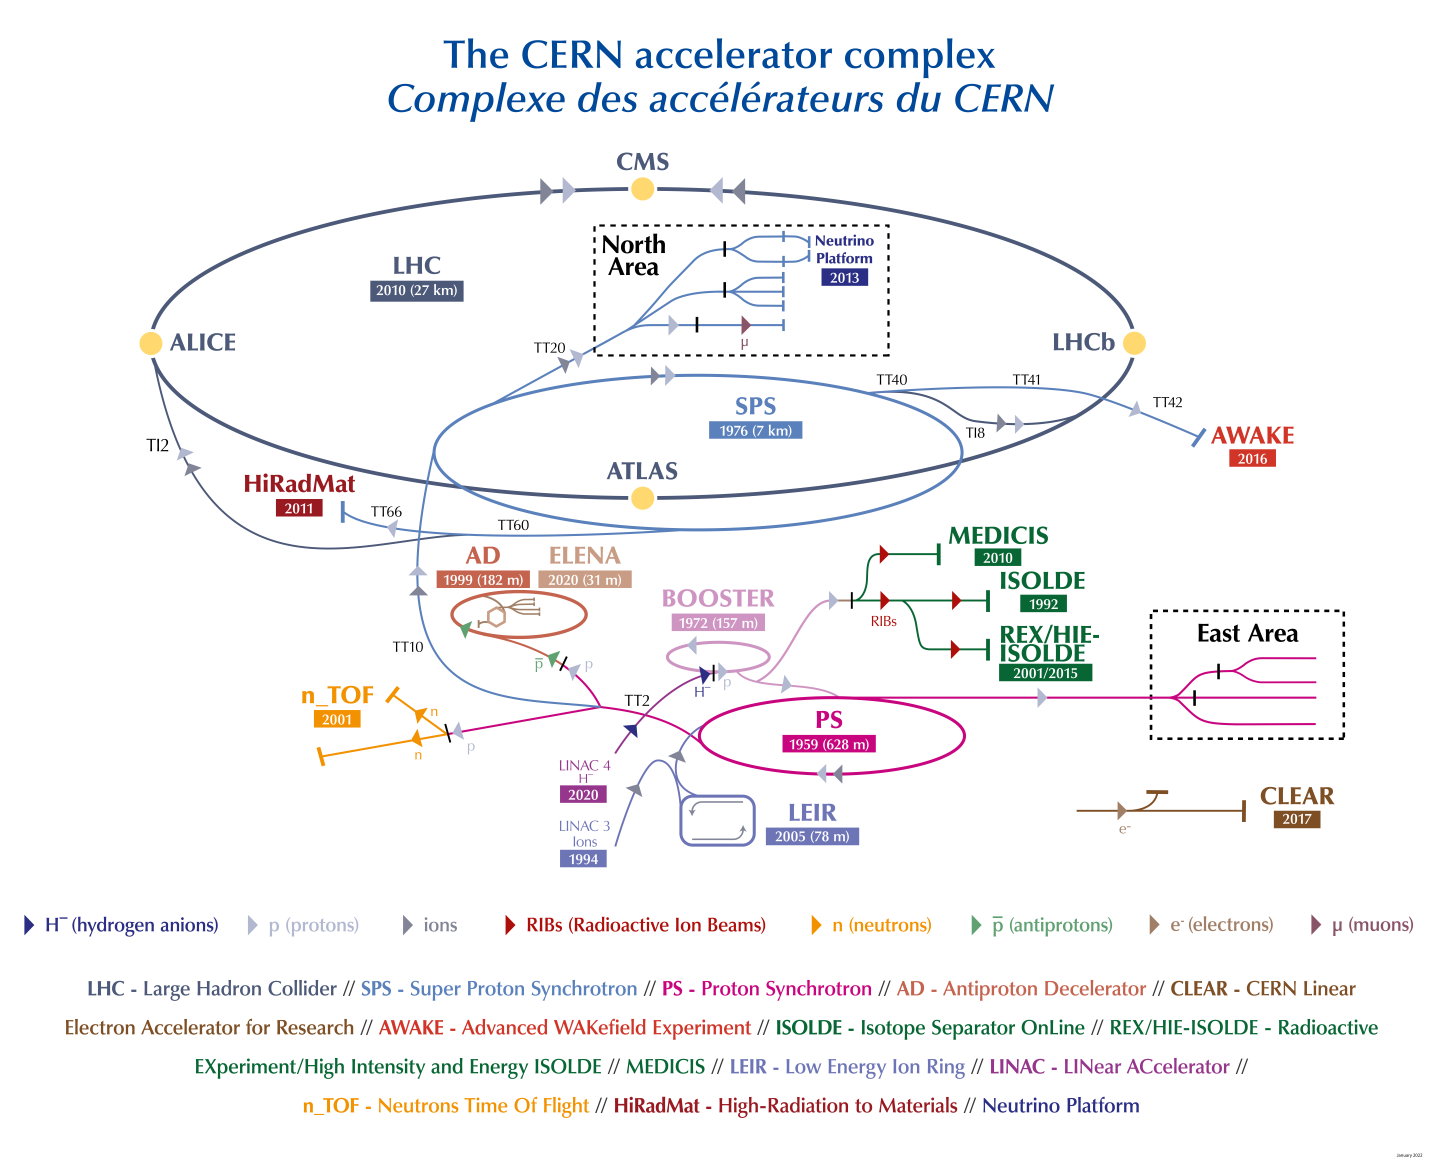
\includegraphics[width=0.8\textwidth]{figures/CCC-v2022.png}\caption{Schematic overview of the CERN accelerator complex.}
\label{fig:cernaccelerators}
\end{center}
\end{figure}

The LHC employs superconducting magnets to bend and focus the particle beams. The machine's 1232 main dipole magnets, each 15 meters in length, operate at 1.9 K using superfluid helium to generate magnetic fields of up to 8.33 T for beam bending. Meanwhile, 392 main quadrupole magnets are used to focus the beams. For acceleration, the RF system utilizes 400 MHz superconducting cavities to provide an energy boost of 16 MV per turn. To ensure the particles don't collide with stray gas molecules, an ultra-high vacuum of $10^{-13}$ atmospheres is maintained.

The beams are organized in a bunch structure, with up to 2808 bunches per beam separated by 25 ns (corresponding to 7.5 m spacing). Each bunch contains approximately $1.15 \times 10^{11}$ protons. The beam energy stored at full intensity reaches 362 MJ per beam, comparable to the kinetic energy of a 400-ton train at 150 km/h.

The LHC has operated at increasing center-of-mass energies: 7 TeV in 2010-2011, 8 TeV in 2012, 13 TeV during Run 2 (2015-2018), and currently 13.6 TeV in Run 3 (2022-2025), representing the highest collision energies ever achieved in a laboratory.

Four main experiments are installed at the LHC collision points: ATLAS (A Toroidal LHC ApparatuS) and CMS (Compact Muon Solenoid), general-purpose detectors designed to explore the full physics potential of the LHC and are located at Points 1 and 5 respectively; ALICE (A Large Ion Collider Experiment), located at Point 2 and specialized in heavy-ion collisions, studying the quark-gluon plasma formed in lead-lead collisions at $\sqrt{s_{NN}} = 5.02$ TeV per nucleon pair; LHCb (Large Hadron Collider beauty), optimized for b-physics, featuring a forward spectrometer designed to exploit the predominantly forward b-quark production in proton-proton collisions, located at Point 8.


\subsection{Luminosity}

Luminosity is a crucial measure of a particle collider's performance. It quantifies the number of collisions per unit time and area, and is therefore directly proportional to the event rate of any given physics process. The event rate for a physics process with cross-section $\sigma$ is given by:
\begin{equation}
R = \mathcal{L} \cdot \sigma,
\end{equation}
where $\mathcal{L}$ is the instantaneous luminosity, typically meaasured in units of cm$^{-2}$s$^{-1}$. For gaussian beams colliding head-on, the instantaneous luminosity can be approximated as:
\begin{equation}
\mathcal{L} = \frac{N_b^2 n_b f_{\text{rev}} \gamma}{4\pi \epsilon_n \beta^*} F,
\end{equation}
where $N_b$ is the number of particles per bunch, $n_b$ is the number of bunches, $f_{\text{rev}} $ is the revolution frequency, $\gamma$ is the Lorentz factor, $\epsilon_n$ is the normalized transverse emittance, $\beta^*$ is the beta function at the interaction point, and $F$ is a geometric factor accounting for the crossing angle. 

To determine the total number of events, $N$, for a process with cross-section $\sigma$ over a given period of time, one must use the integrated luminosity, $\mathcal{L}_\text{int}=\int \mathcal{L} \,dt$:
\begin{equation}
N = \mathcal{L}_\textbf{int} \cdot \sigma.
\end{equation}
The integrated luminosity is typically measured in units of inverse femtobarns (fb$^{-1}$), with 1 fb$^{-1}$ equivalent to 10$^{39}$ cm$^{-2}$.

As of 2025, the LHC Run 3 achieved peak instantaneous luminosities exceeding $2.0 \times 10^{34}$ cm$^{-2}$s$^{-1}$, with ATLAS and CMS each collecting over 100 fb$^{-1}$ of integrated luminosity. Run 3 is scheduled to continue through 2025, with a target of delivering approximately 300 fb$^{-1}$ to each general-purpose experiment.

The High-Luminosity LHC (HL-LHC) upgrade, scheduled to begin operations around 2029, will increase the integrated luminosity by a factor of 10, collecting up to 3000 fb$^{-1}$. This will enable percent-level measurements of Higgs couplings and significantly extend the mass reach for new particle searches.

\section{The ATLAS Experiment}

The ATLAS detector is a general-purpose particle detector at the LHC. Its main goal is to study the fudamental nature of the universe by precisely measuring the properties of particles that are created in high-energy proton-proton collisions. ATLAS is the largest volume particle detector ever constructed, measuring 44 meters in length and 25 meters in diameter, with a total weight of approximately 7000 tons. The detector consists of multiple subsystems arranged in concentric layers around the interaction point, as shown in Figure~\ref{fig:atlas_detector}, each optimized for measuring specific particle properties.

\begin{figure}[!htb]
\begin{center}
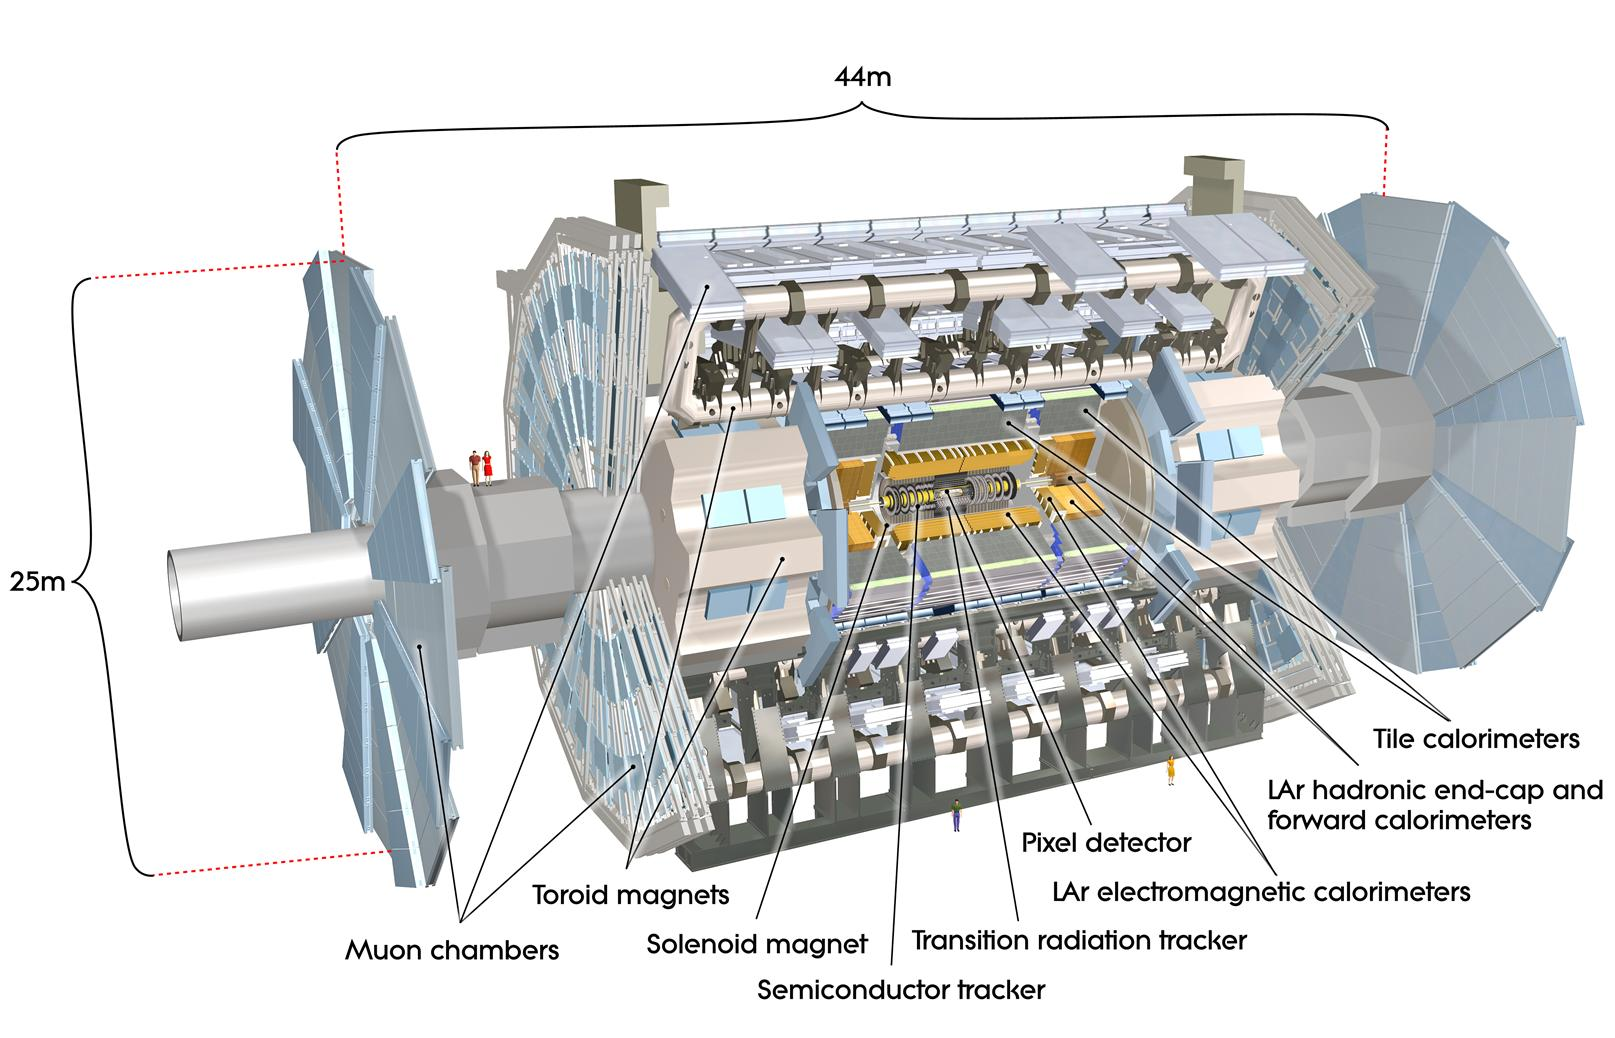
\includegraphics[width=0.8\textwidth]{figures/ATLAS_detector_0803012_01.jpg}\caption{Overview of the ATLAS detector showing all subsystems.} %https://cds.cern.ch/record/1095924 
\label{fig:atlas_detector}
\end{center}
\end{figure}

\subsection{Detector Geometry and Coordinate System}

ATLAS employs a right-handed coordinate system, illustrated in Figure~\ref{fig:atlas_coordinates}, with its origin at the nominal interaction point, chosen to reflect the detector's cylindrical geometry. The $z$-axis points along the beam direction toward the Jura mountains, the $x$-axis points toward the center of the LHC ring, and the $y$-axis points vertically upward. The azimuthal angle $\phi$ is measured in the $x$-$y$ plane from the positive $x$-axis, while the polar angle $\theta$ is measured from the positive $z$-axis.

\begin{figure}[!htb]
\begin{center}
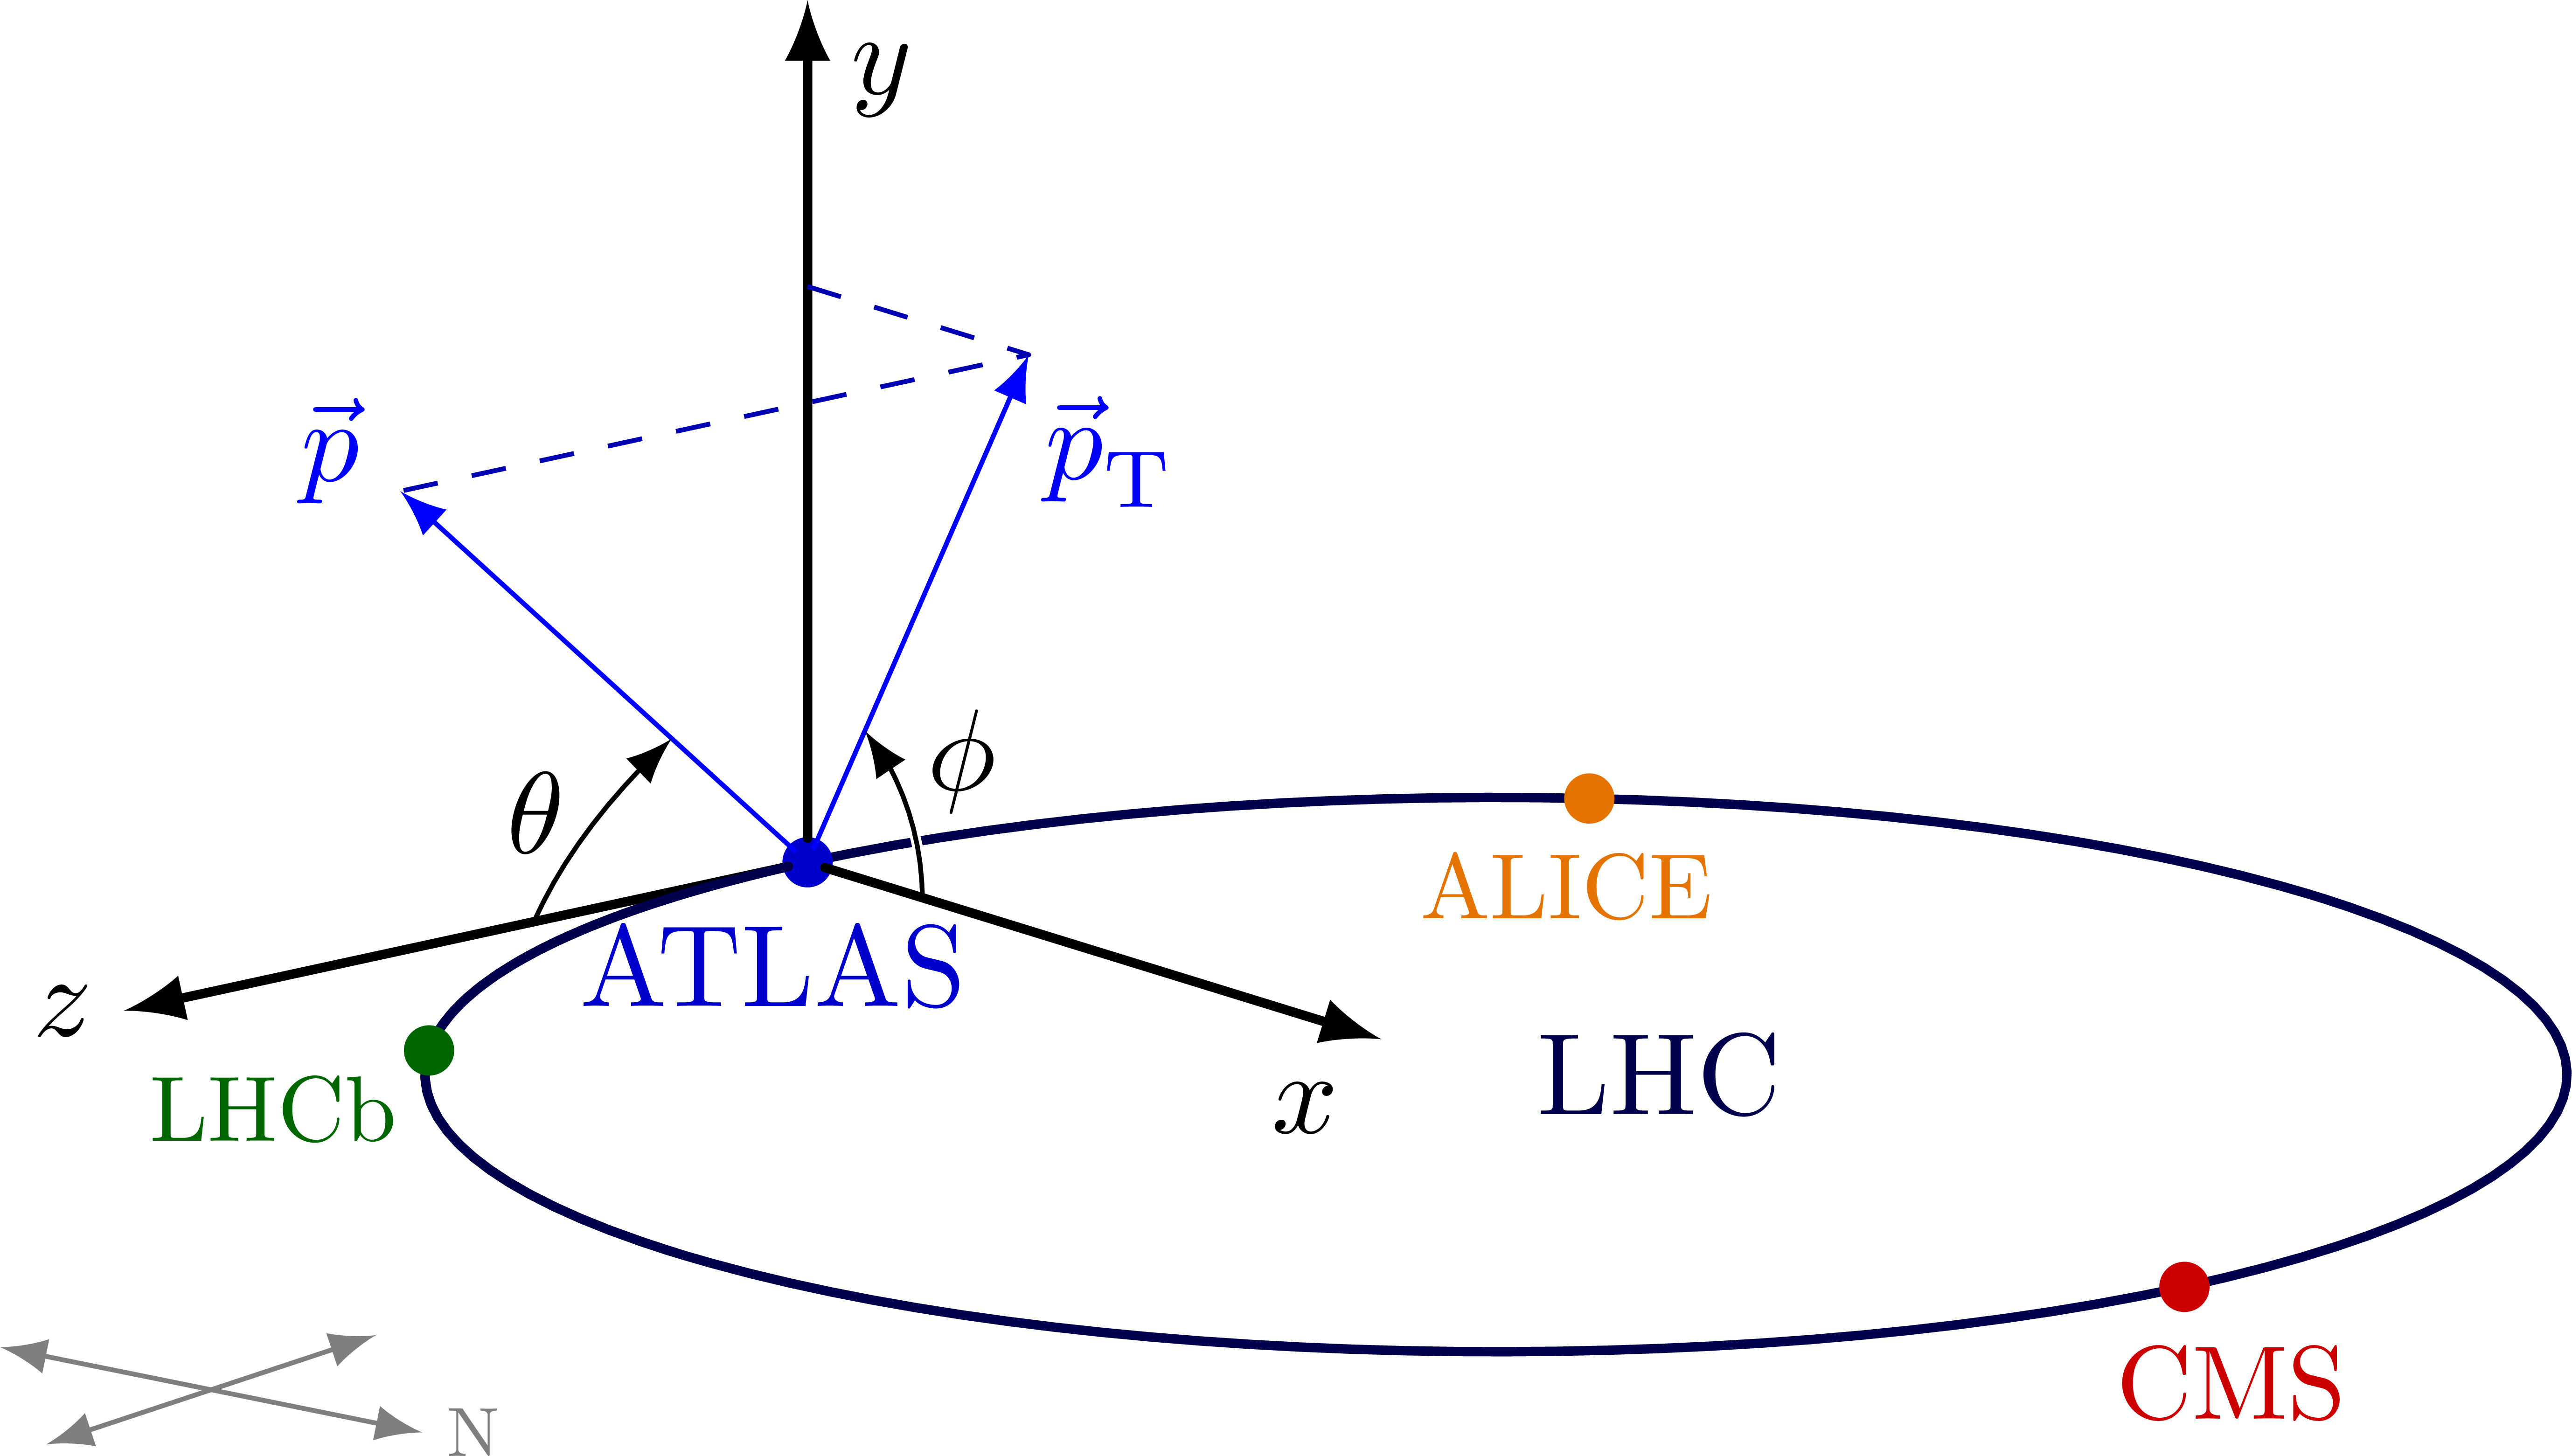
\includegraphics[width=0.8\textwidth]{figures/atlas_coordinate_system.png}\caption{Coordinate system of the ATLAS detector.} %https://tikz.net/axis3d_cms/
\label{fig:atlas_coordinates}
\end{center}
\end{figure}


In hadron collider physics, it is convenient to use the rapidity
\begin{equation}
y = \frac{1}{2} \ln\left(\frac{E + p_z}{E - p_z}\right),
\end{equation}
which transforms additively under longitudinal Lorentz boosts. For highly relativistic particles ($E \gg m$), the pseudorapidity
\begin{equation}
\eta = -\ln\left[\tan\left(\frac{\theta}{2}\right)\right]
\end{equation}
provides a good approximation to the rapidity and depends only on the polar angle.

The angular distance between two objects is typically expressed as
\begin{equation}
\Delta R = \sqrt{(\Delta\eta)^2 + (\Delta\phi)^2}.
\end{equation}

Kinematic variables are often expressed in terms of transverse quantities, because the longitudinal momentum of the colliding partons inside the protons is unknown. The transverse momentum $p_\text{T} = p\sin\theta$ and transverse energy $E_\text{T} = E\sin\theta$ are measured in the plane perpendicular to the beam axis.

The fundamental reason for the importance of these quantities lies in the principle of momentum conservation. While the total longitudinal momentum of the system is unknown, the total transverse momentum before the collision is zero. By the law of conservation of momentum, the vector sum of all transvere momenta of the final-state purticles must also be zero. This conservation principle allows for the calculation of the missing transverse momentum $\vec{p}_\text{T}^\text{miss}$ (with magnitude $E_\text{T}^\text{miss}$). $\vec{p}_\text{T}^\text{miss}$ is defined as the negative vector sum of all detected transverse momenta, indicating the presence of undetected particles such as neutrinos or other non-interacting particles.

\subsection{Inner Detector}

The Inner Detector (ID) is the innermost subdetector of ATLAS, surrounding the beam pipe and contained within a superconducting solenoid that provides a 2 T magnetic field. The ID extends from a radius of approximately 33 mm to 1,080 mm and covers a region of $|\eta| < 2.5$, providing precise tracking of charged particles through the measurement of their trajectories as they curve in the magnetic field.

The ID consists of three systems arranged in concentric cylinders:

\textbf{Pixel Detector:} The innermost tracking system, is positioned as the closest to the interaction point with the first layer (Insertable B-Layer, IBL) at only 33 mm from the beam axis. It's composed of four barrel layers and three end-cap disks per side. It employs approximately 92 million silicon pixels of typical size $50 \times 400$ $\mu$m$^{2}$ (and smaller $50 \times 250$ $\mu$m$^{2}$ pixels in the IBL), and measures 3D space points with high granularity, which is essential for precise vertex reconstruction and identification of $b$-quark jets through displaced vertex tagging.

\textbf{Semiconductor Tracker (SCT):} Surrounding the pixel detector, the SCT uses silicon microstrips with four double layers in the barrel and nine disks per end-cap. The SCT allows for 3D hit reconstruction from 6.3 million readout channels. Each particle typically crosses 8 strip layers. The SCT is designed to extend the tracking volume with a good balance between precision and coverage.

\textbf{Transition Radiation Tracker (TRT):} The outermost tracking component contains 298,000 drift tubes (straws) of 4 mm diameter filled with a Xe/CO$_2$/O$_2$ gas mixture. Particles typically traverse 36 straws. The TRT provides particle identification: when relativistic charged particles cross the polypropylene interfaces between the straws, they produce transition radiation photons, allowing for electron/pion discrimination.


The combined ID achieves a momentum resolution of $\sigma_{p_\text{T}}/p_T = 0.05\%\cdot p_\text{T}[\text{GeV}] \oplus 1\%$ and an impact parameter resolution of 10 $\mu$m for high-$p_\text{T}$ tracks.

\subsection{Calorimeters}

Located immediately outside the solenoid magned surrounding the ID, the ATLAS calorimeter system measures particle energies through total absorption in dense materials. The calorimeters are designed to contain the vast majority of the electromagnetic and hadronic showers while minimizing shower leakage to the muon system.

\textbf{Electromagnetic Calorimeter:} The Liquid Argon (LAr) electromagentic (EM) calorimeter is the primary detector for electrons and photons. Positioned at radii from 1.4 to 2.0 m in the barrel region, it uses liquid argon at 87 K as the active medium with lead absorbers arranged in an accordion geometry. This design provides full $\phi$ coverage without cracks and enables fast signal extraction. The EM calorimeter is divided into a barrel ($|\eta| < 1.475$), end-caps ($1.375 < |\eta| < 3.2$), and forward regions ($3.1 < |\eta| < 4.9$). It features three longitudinal samplings with varying granularity: strips of $\Delta\eta \times \Delta\phi = 0.003 \times 0.1$ in the first layer for $\pi^0/\gamma$ separation, $0.025 \times 0.025$ in the second layer containing most of the shower energy, and $0.05 \times 0.025$ in the third layer. A presampler detector in front of the accordion corrects for energy lost in upstream material. The total depth exceeds 22 radiation lengths ($X_0$) in the barrel. A key upgrade for Run 3 is the new LAr digital trigger electronics. This system significantly improves the granularity of the calorimeter information available at the L1 trigger, by approximately a factor of ten. This allows for a more precise and effective triggering on EM objects in the high pile-up environment.


\textbf{Hadronic Calorimeters:} Three distinct subsystems, each designed to cover a specific region of the detector, are used to measure the energy of hadrons and jets.


\textit{Tile Calorimeter}: Directly outside the EM calorimeter barrel, at radii 2.28-4.25 m, it covers $|\eta| < 1.7$. It is a sampling calorimeter that uses steel plates as the absorber material and scintillating tiles as the active medium. The system is divided into one central long barrel (LB) and two extended barrels (EB), each further segmented into 64 modules in the azimuthal angle. A plug detector, the Intermediate Tile Calorimeter (ITC), is located in the gap/crack region between the LB and EB. The ITC is desinged to measure the energy losses in the dead materials contained in the gap/crack region.

\textit{LAr Hadronic End-cap (HEC)}: Located behind the EM end-caps at $|z| > 4.3$ m, covering $1.5 < |\eta| < 3.2$. This system is also a sampling calorimeter, but with copper plates as the absorbers and liquid argon as the active medium. Its depth of approximately 10 interaction lengths ($\lambda$) is designed to contain most hadronic showers in this region.

\textit{LAr Forward Calorimeter (FCAL)}: Positioned at $|z| = 4.7$ m from the interaction point, covering $3.1 < |\eta| < 4.9$. It is specifically designed to operate in a region with very high particle flux. It uses dense absorber materials (copper for electromagnetic, tungsten for hadronic) and liquid argon as the active medium.

The combined calorimeter system achieves energy resolutions of $\sigma_E/E = 10\%/\sqrt{E[\text{GeV}]} \oplus 0.7\%$ for electromagnetic showers and $\sigma_E/E = 50\%/\sqrt{E[\text{GeV}]} \oplus 3\%$ for hadronic jets.





\subsection{Muon Spectrometer}

The Muon Spectrometer (MS) is the outermost layer of ATLAS, designed to identify and measure the momentum of muons. It extends from approximately 5 m radius in the barrel to 11 m, and reaches $|z| = 21.5$ m in the end-caps. The MS exploits the fact that muons above ~3 GeV are minimum ionizing particles that penetrate the calorimeters with minimal energy loss.

A toroidal magnetic field is generated in the MS by a system of eight rectangular coils in the barrel region (extending from 9.4 to 20.1 m in length) and two additional coils in the end-caps. The superconducting magnets generate magnetic fields of approximately 0.5 T in the barrel and 1 T in the end-caps. This field configuration bends muon trajectories in the $R$-$z$ plane in the barrel and $R$-$\phi$ plane in the end-caps.

For Run 3, the MS uses a combination of precision tracking and fast-response trigger chambers. The most significant upgrade for Run 3 was the replacement of the original Cathode Strip Chambers (CSCs) in the inner end-cap wheels with the New Small Wheels (NSW), which are specifically designed to handle the high background rates of the forward region.

The MS uses four complementary chamber technologies, organized into three distinct stations throughout the barrel and end-caps:


\textbf{Monitored Drift Tubes (MDT):} Provide precision tracking throughout most of the MS volume ($|\eta| < 2.7$). Each tube is 30 mm in diameter, operating with Ar/CO$_2$ gas at 3 bar, achieving 80 $\mu$m single-hit resolution. The chambers are positioned at approximately 5, 7.5, and 10 m radius in the barrel.

\textbf{Resistive Plate Chambers (RPC):} These chambers cover the barrel region ($|\eta| < 1.05$) in three doublet layers. They are fast-response detectors used for the muon trigger, providing a rapid signal with a 25 ns time resolution, and measuring the azimuthal coordinate. Each chamber consists of two resistive plates separated by a 2 mm gas gap. 

\textbf{Thin Gap Chambers (TGC):} Provide triggering in the end-cap region ($1.05 < |\eta| < 2.7$). These multiwire proportional chambers achieve 4 ns time resolution and measure both radial and azimuthal coordinates, with seven layers in the innermost station and three layers in the middle station.

\textbf{New Small Wheels (NSW):} The NSWs cover the region $1.3 < |\eta| < 2.7$, providing both precision tracking and L1 triggers. It consists of two detector technologies: Small-Strip Thin Gap Chambers (sTGC) for fast triggering and precise measurement of the muon's position; and Micromegas (MM) for high-precision trcking for momentum measurement.

The MS achieves a stand-alone momentum resolution of $\sigma_{p_T}/p_T \approx 10\%$ at 1 TeV, which improves to approximately 3\% when combined with ID measurements for muons traversing both systems.


\subsection{Trigger and Data Acquisition}

The ATLAS trigger and Data Acquisition (TDAQ) system is a two-level system that reduces the overwhelming 40 MHz bunch crossing rate to around 3 kHz for permanent storage. This ensures that only events with signatures of potentially interesting physics are saved for offline analysis.

\textbf{Level-1 Trigger (L1):} This is the first stage, hardware-based system, that makes a quick initial decision in just 2.5 $\mu$s. It uses information from the calorimeters and the MS to identify potential physics objects. For Run 3, the L1 trigger has been upgraded to use finer-granularity, digitalized calorimeter data, which allows for more precise object identification. This is further enhanced by the new L1 Topological (L1Topo) processors that apply simple topological selections, to reduce the rate more efficiently. The L1 trigger also integrates information from the NSW to improve the rejection of fake triggers. It reduces the event rate from 40 MHz down to a nominal 100 kHz and identifies Regions of Interest (RoI) for the next stage.

\textbf{High-Level Trigger (HLT):} This second and final stage is a software-based system that processes the events accepted by L1. It runs more sophisticated event reconstruction algorithms, but only on the data within the RoIs identified by L1. The HLT software has been redesigned to be multi-threaded for Run 3, allowing for a much more efficient use of the computing farm. The HLT selects events based on a trigger menu (a dynamic set of criteria and thresholds, optimized for each data-taking period), reducing the rate from 100 kHz to approximately 3kHz for permanent storage.

\textbf{Data Acquisition (DAQ):} The DAQ system manages the flow of data from the detector to the HLT and eventually to storage. When an event is accepted by the L1 trigger, the DAQ reads out the full high-resolution data from all subdetectors. A major upgrade for Run 3 is the new Front-End Link eXchange (FELIX) system. This is a high-throughput network that simplifies the data flow from the detector electronics to the HLT computing farm, making the entire DAQ system more scalable and flexible to handle the increased data volume and rates of Run 3.



\section{Object Identification and Reconstruction}

The identification and reconstruction of physics objects from detector signals is a fundamental step of all ATLAS physics analyses, allowing for the transformation of raw detector data into physics measurements. In Run 3, with average pile-up exceeding 50 interactions per bunch crossing, ATLAS has developed new algorithms that combine data from multiple detector subsystems to ensure that physics object reconstruction and analysis performance are maintained at or exceeding the levels of Run 2.

\subsection{Track and Vertex Reconstruction}

Track reconstruction begins with the formation of space points from hits in the ID silicon detectors. These space points are combined into track seeds, which are subsequently extended and fitted through the entire ID via a combinatorial Kalman filter. Track parameters are described by five quantities $(d_0, z_0, \phi, \theta, q/p)$ defined with respect to the beam spot, where $d_0$ and $z_0$ represent the transverse and longitudinal impact parameters, while $q/p$ denotes the charge-to-momentum ratio.

The primary inside-out tracking pass starts from three-hit seeds in the pixel detector and progressively adds compatible hits from outer layers. An ambiguity resolution algorithm removes duplicate and fake tracks by scoring candidates based on hit patterns, track $\chi^2$, and momentum. For Run 3, the tracking algorithms have been optimized to reduce fake track rates by more than 50\% while maintaining reconstruction efficiency above 99\% for tracks with $p_T > 1$ GeV.

Primary vertex reconstruction uses an iterative vertex finder that identifies the hard-scatter vertex among the multiple proton-proton interactions. The algorithm achieves longitudinal resolution better than 50 $\mu$m for vertices with more than 20 associated tracks, which is crucial for pile-up suppression and object-vertex association.

\subsection{Electron and Photon Reconstruction}

The reconstruction of electrons and photons in Run 3 utilizes dynamic, variable-size superclusters, replacing the fixed-size algorithm of previous runs. Reconstruction begins with topological clusters (topo-clusters) in the electromagnetic calorimeter, which are formed by grouping cells based on their signal significance, defined as the ratio of the cell's energy deposit to its expected noise ($E/\sigma_\text{noise}$). A cell can initiate a clusted (be a ``seed'') if its significance is greather than a set threshold, typically $4\sigma_\text{noise}$.

For electrons, reconstruction involves matching an ID track to a topological calorimeter cluster. To account for energy loss from bremsstrahlung, the track trajectory is refit using a specialized generalized Kalman Filter. The total energy of the electron is then measured by forming a supercluster, which aggregates the main energy deposit (the seed cluster) with smaller, nearby clusters created by bremsstrahlung photons. 

Photons are typically identified as electromagnetic clusters without a matching track. However, photons that convert into an $e^+e^-$ pair in the detector material are reconstructed using dedicated algorithms that find the secondary vertex ot the $e^+e^-$ pair.

Electron and photon identification employs multivariate techniques based on shower shapes, track quality, and transition radiation. The identification efficiencies in Run 3 show uncertainties reduced by 30-50\% compared to Run 2 results. The energy resolution achieved after calibration is on the order of 1-2\% for objects with $E_T > 25$ GeV.

\subsection{Muon Reconstruction}

Muon reconstruction combines measurements from the MS with information from the ID and calorimeters through two complementary strategies. The primary outside-in pass starts from track segments in the MS and matches them with ID tracks that extrapolate from the interaction point. These are then combined into a single, high-quality track, which is refit to account for energy loss.

An inside-out reconstruction chain complements this pass, and it's especially important for reconstructing muons with low $p_\text{T}$ or those in regions with limited MS coverage. This pass begins with a track found in the ID and attempts to extrapolate it outwards. It includes different types of recovered muons, such as ``segment-tagged'' muons, identified by a compatible MS segment, and ``calorimeter-tagged'' muons that leave a minimum-ionizing signature in the calorimeters.

Muon identification criteria range from ``Loose'' to ``Tight'' working points, and are optimized for different physics analyses. Large samples of $Z\to\mu\mu$ and $J/\psi\to\mu\mu$ decays are used for efficiency measurements of reconstruction and identification. The combined momentum resolution reaches $\sigma(p_T)/p_T \approx 2\%$ for muons with $p_T$ around 100 GeV.

\subsection{Jet Reconstruction and Particle Flow}

Starting from Run 3, the particle flow approach is the default method for jet reconstruction in ATLAS, representing a major improvement over traditional calorimeter-based methods. The particle flow algorithm's primary goal is to combine the most accurate measurements from all subdetectors to create a precise and complete reconstruction of each jet. It achieves this by using the highly accurate momentum measurement from the ID for charged particles and the calorimeter energy measurements for neutral particles, effectively avoiding the double-counting of energy.

The algorithm proceeds by first reconstructing tracks in the ID and extrapolating their trajectories to the calorimeter. These extrapolated tracks are then matched to topological clusters based on angular distance and the expected shower profile. For each matched track-cluster pair, the algorithm performs a cell-by-cell energy subtraction from the cluster. This subtraction removes the energy contribution of the charged particle, leaving behind the energy from neutral particles.

The remaining unsubtracted calorimeter deposits, which represent neutral particles (photons and neutral hadrons), are combined with the original charged particle tracks. This complete set of particle flow objects is then used as input to the anti-$k_t$ jet clustering algorithm. This method provides a more precise and complete description of the energy content of the jets.

The particle flow approach provides a 15-20\% improvement in jet energy resolution for jets with $p_\text{T}<70$ GeV compared to calorimeter-only reconstruction. This method is also more stable against the effects of high pile-up due to the precise vertex association of charged particles.

Jet energy scale calibration is performed in multiple stages, including pile-up subtraction, Monte Carlo-based calibration, and data-driven corrections.

\subsection{Heavy-Flavor Tagging}

The identification of jets containing $b$-hadrons (b-tagging) is crucial for many ATLAS physics analyses. It exploits the relatively long lifetime of $b$-hadrons ($c\tau \approx 450$ $\mu$m), which results in displaced decay vertices that are identified in the ID. For Run 3, ATLAS has moved to a new generation of tagging algorithms based on Graph Neural Networks (GNNs), with the GN2 algorithm becoming the new standard.

The GN2 algorithm uses a Transformer architecture to directly process individual track parameters and jet kinematics. In this approach, each track in a jet is treated as a node in a graph. The network analyzes a 23-dimensional feature vector for each track to predict the jet's flavor, while also identifying track origins and vertex associations. This advanced approach provides a significant performance increase over the previous tagger, DL1d. For example, at a 70\% b-tagging efficiency, GN2 improves light-jet rejection by approximately a factor of 2.5 and $c$-jet rejection by approximately a factor of 3.

The performance of b-tagging algorithms is calibrated using data-driven methods. This is tipically done by using large samples of $t\bar{t}$ events for $b$-jets and $D^{*+}$ mesons for $c$-jets.

\subsection{Tau Lepton Reconstruction}

Hadronic tau decays ($\tau_h$) are reconstructed from jets with $p_T > 10$ GeV and $|\eta| < 2.5$. For Run 3, ATLAS uses Recurrent Neural Networks (RNN) based algorithms for tau identification.

The RRN processes both individual tracks and calorimeter clusters to identify tau candidates and reject backgrounds. The RNN is particularly effective at handling the variable track multiplicity of tau decays (one or three charged particles). A dedicated energy calibration, which accounts for the unique shower shape of a tau, is then applied to the candidates using Boosted Regression Trees.

\subsection{Missing Transverse Momentum}

The missing transverse momentum $p_\text{T}^\text{miss}$, with magnitude $E_\text{T}^{\text{miss}}$, quantifies momentum imbalance in the transverse plane of the detector. A non-zero $E_\text{T}^{\text{miss}}$ indicates the presence of undetected particles, such as neutrinos or hypothetical BSM invisible particles, which do not interact with the detector. This measurement relies on the principle of momentum conservation: while the initial longitudinal momentum of the colliding partons is unknown, since the total transverse momentum of the initial colliding system is zero, the total transverse momentum of the final state must also be zero.

The $p_\text{T}^\text{miss}$ vector is calculated by summing the transverse momenta of all reconstructed particle flow objects. The algorithm uses the calibrated momenta of identified electrons, muons, photons and jets, as well as a ``soft term'' that accounts for low-$p_\text{T}$ particles and energy deposits not associated with any reconstructed object. 

The calculation vectorially sums transverse momenta of all particle flow objects, with identified electrons, muons, and photons replaced by their calibrated versions. A soft term accounts for low-$p_T$ particles not associated with reconstructed objects. The pile-up fit algorithm estimates and subtracts pile-up contributions based on spatial energy distributions across the calorimeter.

The $E_T^{\text{miss}}$ resolution scales approximately as $\sigma(E_T^{\text{miss}}) \approx 0.5\sqrt{\Sigma E_T}$ GeV$^{1/2}$, where $\Sigma E_T$ represents the scalar sum of transverse energies of all reconstructed objects. 
\input{chapters/summary.tex}
\input{chapters/summary-swe.tex}

%----------------------------------------------------------------------------
% REFERENCES
%----------------------------------------------------------------------------

\cleardoublepage
\addtocounter{chapter}{1}
\renewcommand{\bibname}{References}
\renewcommand{\ThumbBoxColor}{red}

\newcommand{\RefsBox}{\ThumbBox{Refs}{0}}
\fancypagestyle{plain}
{
   \fancyhead[CE]{\RefsBox}
   \fancyhead[CO]{\RefsBox}
}
\fancyhead[CE]{\RefsBox}
\fancyhead[CO]{\RefsBox}

\bibliographystyle{biblio/JHEP}
\bibliography{biblio/lic-thesis}

%%%%%%%%%%%%%%%%%%%%%%%%%%%%%%%%%%%%%%%%%%%%%%%%%%%%%%%%%%%%%%%%%%%%%%%%%%%%%
% PAPERS
%%%%%%%%%%%%%%%%%%%%%%%%%%%%%%%%%%%%%%%%%%%%%%%%%%%%%%%%%%%%%%%%%%%%%%%%%%%%%

\label{lastPageOfPartI}
\cleardoublepage

\renewcommand{\RefsBox}{}

\fancypagestyle{plain}
{
    \fancyhf{}
    \fancyfoot[LE,RO]{\thepage}
    \renewcommand{\headrulewidth}{0pt}
    \renewcommand{\footrulewidth}{0pt}
}

\fancyhf{}
\fancyhead[LE,RO]{\thepage}

\newcommand{\paperSection}[6]{  % Arguments:
  \def\PaperID{#1}           % ID of the paper I, II, ...
  \def\PaperTitle{#2}        % Title that goes to the table of contents
  \def\PaperInfo{#3}         % Info that goes to the separation page
  \def\PaperFile{#4}         % Filename of the PDF in papers/ folder
  \def\PaperFolioX{#5}       % X position of our folio (page number)
  \def\PaperFolioY{#6}       % Y position of our folio (page number)
  \labelPaper{\PaperID}
  \addtocounter{chapter}{1}
  \pagestyle{plain}
  \phantomsection
  \addcontentsline{toc}{chapter}{\numberline{\hspace{-2mm}\PaperID}\PaperTitle}
  ~ % No text here (everything is in the overlay)
  \ThumbBoxLarge{Paper~\PaperID}{-5}
  \overlayPaperInfo{\PaperInfo}
  \cleardoublepage
}

\newcommand{\includePDF}[1]{
  \ifIncludePDFs
    \pagestyle{empty}
    \includepdf[pages={-}, noautoscale=true, #1,
      pagecommand={
        \noindent\ThumbBox{Paper~\PaperID}{-5}
        \overlayPaperFolio{\thepage}{\PaperFolioX}{\PaperFolioY}
      }]{papers/\PaperFile.pdf}
    \cleardoublepage
  \fi
}

\phantomsection
\addcontentsline{toc}{part}{Part II \;Papers}
\renewcommand{\ThumbBoxColor}{black}

%----------------------------------------------------------------------------
% Paper I
%----------------------------------------------------------------------------

\paperSection{I}
  {Paper title}
{Authors, 
    \emph{Paper title}, 
    [\href{https://arxiv.org/abs/1708.07833}{1708.07833}]}
{1708-07833}{2}{\ifSpaper 8.7 \else 20 \fi}
\label{art:A} % PDF

\renewcommand{\PaperSubFolioFontSize}{10}
\setcounter{PaperSubFolio}{0}

\ifSpaper
  \includePDF{scale=0.96,offset=-2mm 0mm}
\else
  \includePDF{scale=1,offset=2mm 0mm}
\fi

%----------------------------------------------------------------------------
% Paper II
%----------------------------------------------------------------------------

\paperSection{II}
  {Paper title}
  {Authors, 
    \emph{Paper title}, 
    [\href{https://arxiv.org/abs/1708.07833}{1708.07833}]}
  {1708-07833}{2}{\ifSpaper 8.7 \else 20 \fi}
\label{art:B}

\renewcommand{\PaperSubFolioFontSize}{10}
\setcounter{PaperSubFolio}{0}

\ifSpaper
  \includePDF{scale=0.96,offset=-2mm 0mm}
\else
  \includePDF{scale=1,offset=2mm 0mm}
\fi

%----------------------------------------------------------------------------
% Paper III
%----------------------------------------------------------------------------

\paperSection{III}
  {Paper title}
{Authors, 
    \emph{Paper title}, 
    [\href{https://arxiv.org/abs/1708.07833}{1708.07833}]}
{1708-07833}{2}{\ifSpaper 8.7 \else 20 \fi}
\label{art:C}

\renewcommand{\PaperSubFolioFontSize}{10}
\setcounter{PaperSubFolio}{0}

\ifSpaper
  \includePDF{scale=0.87,offset=-2mm 0mm}
\else
  \includePDF{scale=0.98,offset=1mm 0mm}
\fi

%%%%%%%%%%%%%%%%%%%%%%%%%%%%%%%%%%%%%%%%%%%%%%%%%%%%%%%%%%%%%%%%%%%%%%%%%%%%%
% Show LAYOUT INFO (optional)
%%%%%%%%%%%%%%%%%%%%%%%%%%%%%%%%%%%%%%%%%%%%%%%%%%%%%%%%%%%%%%%%%%%%%%%%%%%%%

\pagestyle{empty}

\ifShowLayout
  \setcounter{chapter}{1}
  \phantomsection
  \renewcommand*{\FrameEdgeColor}{blue!40}
  \renewcommand*{\ShowSubGridColor}{gray!40}
  \renewcommand*{\ShowGridColor}{gray!70}
  \renewcommand*{\ShowFrameColor}{\color{red!40}}
  \renewcommand*{\ShowGridTextColor}{gray}
  % \renewcommand*{\ShowFramePicture}{}
  \AddToShipoutPictureBG{
     \ThumbBoxLarge{Paper~L}{0}
     \ThumbBox{Tab 5}{4}
     \ThumbBox{Tab 10}{9}
  }
  \noindent
  % \textsf{\textbf{Layout info}}\\[2mm]
  \setvaluestextsize{\footnotesize}
  \footnotesize
  \printinunitsof{mm}{\pagevalues}\\
  ~\verb| \marginparwidth| = 
  \printinunitsof{mm}\prntlen{\marginparwidth}
  ~\verb|   \TopOffset| = 
  \printinunitsof{mm}\prntlen{\TopOffset}\\
  ~\verb| \FontSize| = \FontSize
  \ifSpaper
     \setlayoutscale{0.45}
  \else
     \setlayoutscale{0.5}
  \fi
  \pagediagram
  \setvaluestextsize{\normalsize}
  \normalsize
\else
  ~
\fi

\end{document}
